\part{Experimental control}
\label{part:experiment}

\chapter{Experimental Testbed and Experiment Engines}%
\label{chapter:experiment:testbed}

    \section{State of the art}%
    \label{sec:state_of_the_art}

        \subsection{Grid'5000}%
        \label{sub:grid_5000}

            Nearly all the experiments presented in this document have been carried on the Grid'5000~\cite{grid5000}
            testbed.  Quoting its official website\footnote{\url{https://www.grid5000.fr/}}: \blockquote{Grid'5000 is a
            large-scale and flexible testbed for experiment-driven research in all areas of computer science, with a
            focus on parallel and distributed computing including Cloud, HPC and Big Data and AI.} It provides dozen of
            clusters, each one having between 2 and 124 homogeneous compute nodes. There is a high diversity of hardware,
            including several generations of Intel processors available, AMD and ARM processors, GPU, persistent memory
            (PMEM) as well as high-performance networks such as Infiniband or Omni-path. Another important feature is the
            ability for the experimenter to get full control on the nodes, as it is possible to deploy a new operating
            system and therefore to gain superuser access.

        \subsection{Experiment engines}%
        \label{sub:experiment_engines}

            While it is possible to run a complete experiment on a testbed like Grid'5000 by manually issuing commands
            in an interactive shell, it is not advisable as it quickly becomes extremely tedious and error-prone.
            Automating the experiment is a necessary condition to have reproducible results. A first step toward this
            goal is to write some ad-hoc script. However, two independent experiments might still share a lot of steps
            that could be refactored in a common layer, \eg OS deployment, package installation, or even more advanced
            features like node instrumentation or environment logging.

            For these reasons, it is a common practice to use an experiment engine. Buchert~\etal describe the features
            of eight different engines~\cite{buchert:hal-01087519}. To the best of our knowledge, only three offer a
            native support for Grid'5000, namely Expo, XPFlow and Execo. Unfortunately, Expo and XPFlow are now longer
            maintained, the last commit in their respective repositories was done on November 2014 and September 2015
            For these reasons, the experiment engine Execo~\cite{Imbert_2013} is often recommended to Grid'5000
            newcomers.

            Experiments with Execo are described as a Python script. We believe this is one of its best qualities, as it
            offers a lot of freedom and flexibility to the experimenter, comparatively to other experiment engines that
            use custom domain specific languages (DSL). Yet, we made the choice to not use it. The main reason is that a
            typical Execo experiment uses a lot of low-level constructs that are really unpleasant and unintuitive to
            write and read. Section~\ref{sub:comparison_with_execo} will present some comparisons. Furthermore, Execo
            lacks a lot of important features, like node instrumentation and metadata collection, \ie we would still
            have needed to implement a lot functionalities on top of Execo.

    \section{Yet another experiment engine: \texttt{peanut}}%
    \label{sec:peanut}
        %% TODO
        %% Différents moyens mis en oeuvre pour faciliter la reproductibilité (au sens
        %% large) :
        %% - Description structurée et lisible d'une expérience, relativement haut niveau
        %%   -> on comprend facilement ce qu'il se passe, on peut reproduire l'expérience
        %%   sans utiliser peanut.
        %% - Une fois l'expérience écrite, 100% automatisé, lancée avec juste une ligne de
        %%   commande.
        %% - Collecte d'information : commandes exécutées et leur std{out,err},
        %%   informations système, timestamps, monitoring.
        %% - Attention aux excès, pas forcément pertinent de collecter 10GB
        %%   d'info par expérience, voir même contre-productif si ça incite à ne
        %%   pas refaire les XP. Parler des problèmes découverts sur G5K (ref. au
        %%   dernier chapitre) ?
        %% - Future work: NIX & GUIX.
        %% - L'utilisateur garde le contrôle sur le plan d'expérience, grâce à des fichiers
        %%   d'expériences (peanut n'est pas chargé de randomiser l'xp). Ref à la prochaine
        %%   section.
        \subsection{Key features}%
        \label{sub:key_features}
            We implemented our own experiment engine, named \texttt{peanut}. It comes as a Python library that
            experimenters can use to write their own experiments, also as a Python script.

            A new experiment can be defined by inheriting from the class \texttt{peanut.Job}. Three methods can be
            overridden, \texttt{setup}, \texttt{run\_exp} and \texttt{teardown}.

            Once the experiment is written, it can be launched in a single command line. The following steps will
            happen.
            \begin{itemize}
                \item Implicitly, submit a job with the given characteristics (\eg cluster, number of nodes, walltime,
                    etc), then deploy the given OS image.
                \item Implicitly (but optionally) enable or disable some performance functionalities like
                    hyperthreading, turboboost, C-states.
                \item Implicitly (but optionally) instrument the nodes to collect at a regular interval some system
                    metrics (\eg core frequencies and temperatures, CPU power consumption, network traffic, memory
                    consumption).
                \item Implicitly (but optionally) run the \texttt{stress} command on all the nodes to warm them up.
                \item Run the methods \texttt{setup}, \texttt{run\_exp} and \texttt{teardown} in that order.
                \item Produce a \texttt{zip} archive containing relevant results and metadata. The experimenter can
                    explicitly add any file to the archive. In addition, the following content is also implicitly
                    archived:
                    \begin{itemize}
                        \item Metrics collected with the aforementioned instrumentation.
                        \item Human-readable log of the commands issued during the experiment.
                        \item Machine-parsable log of the commands (in JSON format) with their timestamps and output
                            (both \texttt{stdout} and \texttt{stderr}).
                        \item Machine-parsable file (in Yaml format) containing relevant information like
                            the exact versions used for \texttt{peanut}, \texttt{gcc}, \texttt{MPI} and the Linux
                            kernel, the command line that was used to launch this experiment, the cluster and the list
                            of nodes, start and end timestamps for each of the three main methods, the list of the git
                            repositories cloned during this experiment with their remote URL and the git hash of the
                            checkout.
                        \item For each node, the content of the file \texttt{/proc/cpuinfo} as well as the output of the
                            commands \texttt{env}, \texttt{lstopo}, \texttt{lspci}, \texttt{dmidecode},
                            \texttt{lsmod}, \texttt{dmesg}.
                    \end{itemize}
            \end{itemize}
            In addition, the experiment can be executed interactively in a Python terminal. All the implicit
            : functionalities described previously can also be explicitly called (\eg there are methods
            \texttt{disable\_hyperthreading}, \texttt{start\_monitoring} and \texttt{perform\_stress}).

            An experiment can be parametrized by two means:
            \begin{itemize}
                \item An install file. This is a Yaml file that can be used to describe how the setup phase should be
                    done. Typically, it can contain the desired version for different libraries like OpenBLAS or
                    OpenMPI, but also the duration of the warmup or the frequency of the monitoring.
                \item An experiment file. These can be of any kind. A typical use case is to provide a CSV file where
                    each line is a particular piece of the experiment (\eg an individual call to \dgemm and the
                    columns represent the parameters for these experiments (\eg the sizes \texttt{M}, \texttt{N} and
                    \texttt{K} used by \dgemm).
            \end{itemize}

        \subsection{Comparison with Execo}%
        \label{sub:comparison_with_execo}

            In this section, we use a small example to illustrate some differences between \texttt{peanut} and
            \texttt{execo}. The goal is to write an experiment that will take several nodes on a given Grid'5000
            cluster, compile the \texttt{CRoaring} library\footnote{\url{https://github.com/RoaringBitmap/CRoaring}} and
            run one of its benchmarks.

            \lstdefinestyle{custom_lst_style}{
             %   language=Matlab,
                numbers=left,
                stepnumber=1,
                numbersep=10pt,
                tabsize=4,
                showspaces=false,
                showstringspaces=false
            }
            \lstset{basicstyle=\scriptsize, style=custom_lst_style}

            First, Listing~\ref{lst:engine:execo} shows such an experiment using Execo. Run with: \verb#python script.py#\\

            \lstinputlisting[language={Python},label={lst:engine:execo},
                caption={Small experiment example Execo}]{
                img/experiment/engine/mweExeco.py
            }

            This script, albeit fairly small, is already difficult to read in some places. For instance, lines 11-12,
            one has to write a complex query as a string as follows:

            \verb#OarSubmission("{cluster in ('dahu')}/nodes=2,walltime=00:20:00")#

            It would be much more pleasant to write it as follows:

            \verb#OarSubmission(cluster="dahu", nodes=2, walltime="00:20:00")#

            Now, Listing~\ref{lst:engine:peanut_class} demonstrates how the same experiment can be rewritten using Peanut
            in a much more concise and readable way.

            Run with: \verb#peanut script.py run tocornebize --deploy debian9-x64-base \#\\
            \verb#    --cluster dahu --nbnodes 2 --walltime 00:20:00#

            \lstinputlisting[language=Python,label={lst:engine:peanut_class},
                caption={Small experiment example using Peanut}]{
                img/experiment/engine/mwePeanut.py
            }

            The script is not only twice shorter, it is also much more elegant. Furthermore, it accomplishes much more
            than Listing~\ref{lst:engine:execo}, as it produces a peanut archive with all the metadata related to the
            experiment.

\chapter{On the difficulties of experimentation}%
\label{chapter:experiment:difficulties}
    %% TODO
    %% Calibration experiments: randomisation. pour quoi faire ?
    %% 1. éviter les biais (randomisation de l'espace de paramètres)
    %%    - certaines valeurs peuvent être particulières et on peut vouloir
    %%      au contraire biaiser vers ces valeurs
    %% 2. éviter les perturbations transientes
    %%    - montée en charge vs. régime stationnaire
    %%
    %% Plusieurs exemples à citer (ref aux présentations qu'on aurrait dû
    %% faire à XUG@Rennes et à JLESC@Bonnes).
    Suppose some researcher wants to evaluate the memory bandwidth of their laptop. A first way to answer this question
    could be to write a small program that allocates a buffer, then write some data on this buffer with the
    \texttt{memset} function while measuring the duration of this operation. The problem is that the time taken to make
    this memory write may not be representative, the following writes would very probably have different durations due
    to cache effects.  Therefore, it would be better to make several measures that should then be carefully analyzed
    (maybe simply taking the average, or perhaps there are some \emph{outliers} that should be removed). However, by
    doing so we only measure the performance of a write for a given size. The effective bandwidth could be very
    different with a smaller or a larger buffer. The natural solution here is to repeat these sequences of measures for
    several sizes.

    A general advice shared by experimental scientists in such situations is to randomize the experiments. In general,
    this randomization should happen for:
    \begin{itemize}
        \item The parameter space (in this example, the set of sizes that are evaluated). The goal is to avoid bias, for
            instance sizes that are a power of two may lead to a different performance. Note that in some occasions, as
            this chapter will illustrate, it is desirable to bias the experiment towards some particular values.
        \item The experiment order (in this example, the order of the sizes). The rational here is to avoid temporal
            perturbations. In particular, there are often at least two phases, a load build up which converges toward a
            steady state. There can also be changes that happen once the steady state is reached, \eg caused by some
            external source. By randomizing the order of the experiments, it becomes much easier to recognize an
            eventual temporal perturbation simply by plotting the data.
    \end{itemize}

    In this chapter, we will discuss several lessons learned for conducting faithful experiments, most of the time the
    hard way.

    \section{Experimental setup}%
    \label{sec:experimental_setup}

        All the experiments presented in this chapter share a common setup. They have been repeated on several nodes and
        follow the same steps:
        \begin{enumerate}
            \item Deploy and install a fresh OS on the node.
            \item Run the \texttt{stress} command for 10 minutes to warm the node.
            \item Start a background process\footnote{\url{https://github.com/Ezibenroc/ratatouille}} to monitor the
                core frequencies and temperature every second.
            \item On each core, run a custom
                code\footnote{\url{https://github.com/Ezibenroc/platform-calibration/src/calibration}}
                to measure the durations of a given operation (either \dgemm or several MPI functions, depending
                on the experiment).
        \end{enumerate}

        Unless specified otherwise, we used nodes from the Dahu cluster from
        Grid'5000\footnote{\url{https://www.grid5000.fr/w/Grenoble:Hardware}}. Each of these nodes has two Intel Xeon
        Gold 6130 CPU, which are 16 core CPU from the Skylake generation. They have a base frequency of
        \NSI{2.1}{\giga\hertz} and a turbo frequency of up to \NSI{3.7}{\giga\hertz}, but their turbo frequency is
        limited to \NSI{2.4}{\giga\hertz} when their 16 cores are active and in AVX2
        mode\footnote{\url{https://en.wikichip.org/wiki/intel/xeon\_gold/6130}}. We have used
        OpenBLAS\footnote{\url{https://github.com/xianyi/OpenBLAS}} version~0.3.1 and
        OpenMPI\footnote{\url{https://github.com/open-mpi/ompi}} version~2.0.2 compiled with GCC version~6.3.0 on a
        Debian~9 installation with kernel version~4.9.0.

    \section{Defining the parameter space}%
    \label{sec:parameter_space}

        Two families of experiments are discussed in this chapter: (1) MPI operations such as calls to
        \recv or \send, their duration is proportional to \(S\), the size of the buffer that is
        being communicated, and (2) calls to the \dgemm function, whose duration is proportional to the product
        of the sizes \(MNK\) but also depends on individual interactions of those sizes.

        An experiment consists in a sequence of calls to the function of interest, with various sizes as parameters. The
        goal of this section is to discuss how and why the parameters of these sequences are generated.

        \subsection{MPI communications}%

            If we assume that the duration of a communication is linear in the amount of data being sent, the easiest
            way to sample the data is to only measure two sizes, one very small buffer (\eg \NSI{1}{\byte}) and one very
            large buffer (\eg \NSI{1}{\giga\byte}). To avoid any bias, we could even try several small and large
            buffers with slight differences in their respective sizes. However, we saw in Part~\ref{part:prediction}
            that this linearity assumption does not hold, their are large discontinuities. We therefore need to also
            sample sizes between the two extreme values to (1) make sure that all the breakpoints are visible in our
            dataset and (2) perform one linear regression in each linear zone.

            Given this requirement, the natural sampling method would be a uniform sampling, taking
            \(S\sim\unif{1}{10^9}\). However, in our experiments, we found out that the breakpoints are not uniformly
            spread, but rather exponentially. For instance, the \send on the dahu cluster has four
            breakpoints: \NSI{8.14}{\kilo\byte}, \NSI{34.0}{\kilo\byte}, \NSI{63.8}{\kilo\byte} and
            \NSI{285}{\mega\byte}. If the sizes of the experiment were uniformly sampled, we would very probably miss
            the smaller breakpoints: by sampling uniformly and independently 1000 numbers in the interval \([1, 10^9]\),
            the probability to have at least one number smaller or equal to \(10^5\) is a bit less than
            \NSI{10}{\percent}. The reason for these exponentially spread breakpoints likely comes from the hardware.
            Typically, each layer of the memory hierarchy is one order of magnitude larger than the previous layer. For
            instance, each core of a dahu node has \NSI{32}{\kibi\byte} L1 instruction and data caches and one
            \NSI{1}{\mebi\byte} L2 cache. Then, the 16 cores of a same CPU share a \NSI{22}{\mebi\byte} L3 cache and
            a \NSI{93}{\gibi\byte} memory.

            For these reasons, we made the choice to sample the sizes exponentially in the considered interval. More
            precisely, each size $S$ is sampled as: \[S\sim10^{\unif{0}{9}}\]

        \subsection{Function \dgemm}%
        \label{sub:parameter_space:dgemm}

            The situation is different with the \dgemm function. We did not observe any breakpoint in the performance
            plots as for the MPI communications. Hence, we did not have any reason to use an exponential sampling. A
            first solution would therefore consist in taking \(M=N=K\) and sampling the product \(MNK\) uniformly in
            some interval.  This could be sufficient for a simple linear regression with only one parameter, but as
            discussed in Part~\ref{part:prediction} we need several coefficients of the polynomial. For this reason, we
            have to cover a larger zone of the parameter space.

            Two options have been considered. Suppose we would like the three sizes \(M,N,K\) to be smaller or equal to
            some constant \(\Sigma\) and their product \(MNK\) to be smaller or equal to some other constant \(\Pi\).
            \begin{description}
                \item[Independent sizes] Each of the three sizes \(M\), \(N\) and \(K\) is sampled independently and
                    uniformly in the desired interval:
                    \begin{enumerate}
                        \item \(M \sim \unif{1}{\Sigma}\) and \(N \sim \unif{1}{\Sigma}\) and
                            \(K \sim \unif{1}{\Sigma}\)
                        \item Repeat until \(MNK \leq \Pi\)
                        \item Return \((M,N,K)\)
                    \end{enumerate}
                    This is the easiest method to implement. With this approach, the product
                    \(MNK\) is not uniform, it is heavily skewed towards the small values. Additionally, we use rejection
                    sampling to make sure that the product of the sizes does not get too large.
                \item[Uniform product] We start by sampling the size product \(P\) uniformly in the desired interval,
                    then the sizes \(M\), \(N\) and \(K\) are sampled randomly to get (approximately) the correct
                    product:
                    \begin{enumerate}
                        \item \(P \sim \unif{1}{\Pi}\)
                        \item \(A \sim \unif{1}{\sqrt[3]{P}}\)
                        \item \(B \sim \unif{1}{\sqrt{\frac{P}{A}}}\)
                        \item \(C = \frac{P}{AB}\)
                        \item Repeat steps 2 to 4 until \(A \leq \Sigma\) and \(B \leq \Sigma\) and \(C \leq \Sigma\)
                        \item Return the six possible permutations: \((M,N,K) = (A,B,C), (C,A,B), \dots\)
                    \end{enumerate}
                    The goal of returning all the permutations of the sizes is to avoid any bias in the sampling
                    procedure, since they are not generated independently from each other. We also use rejection
                    sampling to make sure that one of the sizes does not get too large.
            \end{description}

            These two generation methods are illustrated in Figure~\ref{fig:parameter_space}. A list of \Num{100000}
            size tuples was sampled with each approach.

            \begin{figure}[htpb]
                \centering
                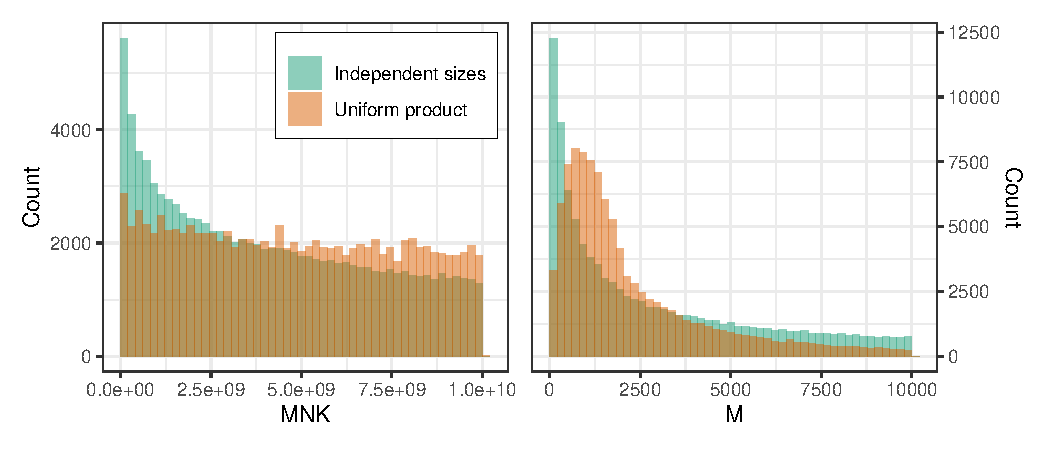
\includegraphics[width=\linewidth]{img/experiment/parameter_space/distribution.pdf}
                \caption{Distribution of the product \(MNK\) and the size \(M\) with the two generation methods. The
                maximal product is set to \(10^{10}\) and the maximal size to \Num{10000}.}%
                \label{fig:parameter_space}
            \end{figure}

            The left plot shows that as expected, the product \(MNK\) appears to have a large left-skew with the first
            approach and to be uniformly distributed with the second approach. The right plot is more surprising, since
            the parameter \(M\) is not uniformly distributed with the first approach. The reason is the rejection
            sampling, large values for \(M\) are more likely to give a product \(MNK\) above the specified limit and
            thus to be rejected.

            Since the product \(MNK\) is the most significant factor for the duration of \dgemm, it is more natural to
            use a uniform distribution for this term, we therefore made the choice to use the second approach for
            generating experiment files for the \dgemm experiments, with two minor modifications:
            \begin{itemize}
                \item Instead of sampling the product uniformly with \(MNK\sim\unif{1}{S}\), we made the choice to use a
                    slightly more deterministic approach. We first compute $\gamma$ different values that are uniformly
                    but deterministically spread in the given interval, \ie we compute the set
                    \(\left\{S, S-\frac{S}{\gamma},S-2\frac{S}{\gamma}, \dots\right\}\)
                    (typically, \(\gamma=30\)). Then we add a random noise independently to each of these sizes. The
                    goal is to ensure a similar (yet still random) distribution of the products \(MNK\) each time we
                    generate a new experiment file. This approach is similar to latin hypercube sampling (LHS).
                \item In addition of the size tuples randomly generated, we systematically add a few tuples to the list,
                    like \((1,1,1)\) or \((2048,2048,2048)\). The goal is to ensure that we have a few identical calls to
                    \dgemm in every experiment, in case we want a fine comparison.
            \end{itemize}

    \section{Randomizing the order}%
    \label{sec:randomizing_order}
        The network model in SMPI needs to be instantiated with a careful calibration of the MPI communication
        performance, as presented by Degomme~\etal \cite{smpi}. This was done with a MPI program created by the Simgrid
        team that performed a sequence of measures with two hosts. Several kind of measures were implemented: the
        \emph{recv} (a call to \recv with waiting to avoid late senders), the \emph{isend} (a call to
        \texttt{MPI\_Isend}), the \emph{pingpong} (a call to \send followed by a call to \recv to get the round-trip
        time) as well as several more minor MPI primitives.

        \begin{algorithm}[H]
            read the sequence of sizes \(S_1\), typically \(|S_1| \approx 1000\)\;
            \(S_2 := \underbrace{S_1\cdot S_1\cdot\dots\cdot S_1}_{N\text{ concatenations, typically } N\approx 50}\)\;
            \For{each kind of measure (recv, isend, pingpong, etc.)}{
                \For{\(s \in S_2\)}{
                    perform the measure $K\approx10$ times and output each individual duration
                }
            }
        \end{algorithm}

        Although the sequence of sizes \(S_1\) is a random sequence, there are still two obvious biases in this
        experiment.  First, the final sequence \(S_2\) is a concatenation of several instances of \(S_1\), so the same
        (random) order will be used in these \(N\) runs. Then, the different kind of measures are performed one after
        the other.

        In a first step towards a better methodology, we started by shuffling entirely the sequence \(S_2\) after the
        concatenation. The observed durations for function \recv with both methods are presented in
        Figure~\ref{fig:randomizing_order:raw_data}. There is no obvious difference here, in both cases the duration is
        piecewise linear in the message size and several modes are present for the small and medium messages.

        \begin{figure}[htpb]
            \centering
            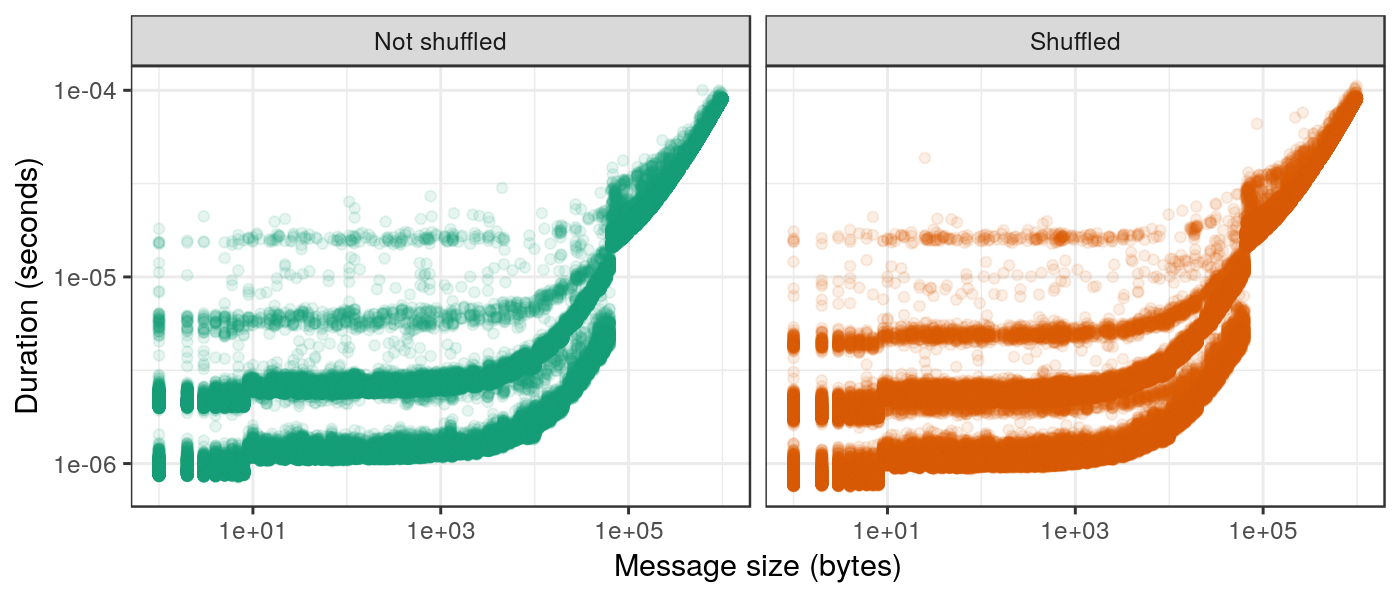
\includegraphics[width=\linewidth]{img/experiment/randomizing_order/raw_data.png}
            \caption{The duration of \recv is piecewise linear, with several modes for small messages.}%
            \label{fig:randomizing_order:raw_data}
        \end{figure}

        To compute a network model for SMPI, we need to perform a (segmented) linear regression on this data. One
        assumption for the simple least-square regression is that the noise should be normally distributed, which is
        clearly not the case with our dataset, the noise is multi-modal. One simple solution for this is to compute the
        average duration for each message size, which all have a large number of measures (500 in this figure). With the
        central limit theorem, assuming that the measures for similar message sizes are independent and identically
        distributed, their sample average is normally distributed. This means that by averaging the data, we should get a
        normal noise which would allow us to compute a linear regression.

        \begin{figure}[htpb]
            \centering
            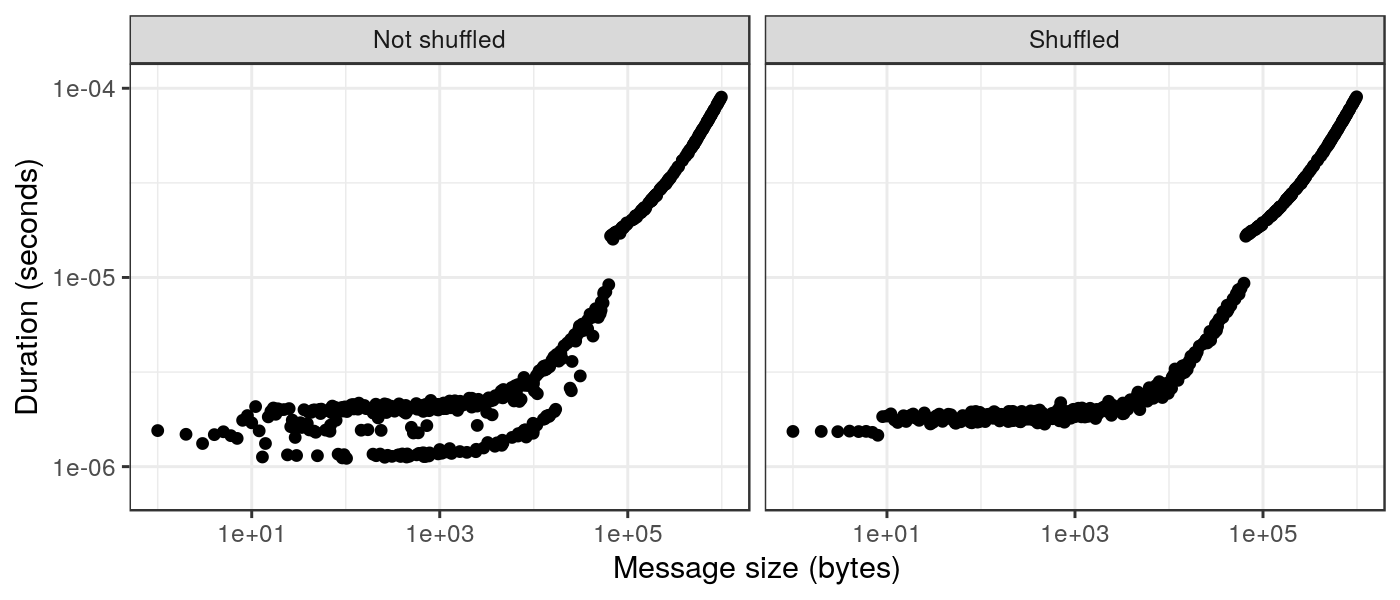
\includegraphics[width=\linewidth]{img/experiment/randomizing_order/aggregated_data.png}
            \caption{The average durations of \recv in the non-shuffled case still show several modes,
            which should not happen according to the central limit theorem.}%
            \label{fig:randomizing_order:avg_data}
        \end{figure}

        The aggregated data is presented in Figure~\ref{fig:randomizing_order:avg_data}. With the shuffled experiment
        (right plot), the average durations have a single-mode, as expected. However, in the non-shuffled case (left
        plot), at least two modes are clearly present. This contradicts the conclusion of the central limit theorem,
        thereby proving that its hypotheses do not hold for this experiment. This is confirmed by
        Figure~\ref{fig:randomizing_order:distribution}, where we zoomed on a few distinct message sizes between
        \NSI{700}{\byte} and \NSI{800}{\byte}. Each point is the duration of an individual call to \recv,
        the crosses represent the average durations. In the shuffled experiment, on the right, the duration
        distributions are similar for all message sizes, with two modes clearly identifiable and the average in between.
        In the non-shuffled case, on the left, the durations of three message sizes are different, namely
        \NSI{703}{\byte}, \NSI{767}{\byte} and \NSI{779}{\byte}. For these three calls, the distributions have only one
        mode, so their average durations are significantly shifted. The assumption of identical distribution for these
        different message sizes is clearly not satisfied here.

        \begin{figure}[htpb]
            \centering
            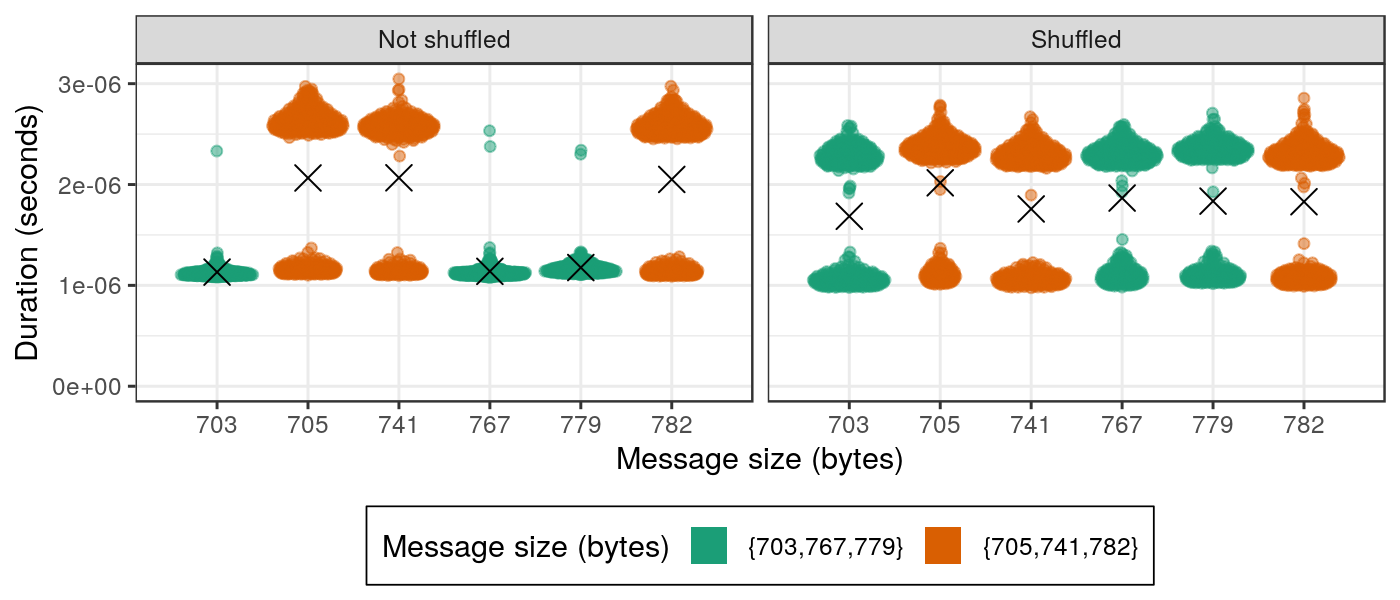
\includegraphics[width=\linewidth]{img/experiment/randomizing_order/distribution.png}
            \caption{Distribution of the \recv durations for six different message sizes between \NSI{700}{\byte} and
            \NSI{800}{\byte}.  The durations are not identically distributed in the non-shuffled case.  Durations
            truncated to \NSI{4}{\micro\second} for a better readability.}%
            \label{fig:randomizing_order:distribution}
        \end{figure}

        Since shuffling correctly the experiments prevents the occurrence of this issue, a possible reason could be that
        the individual calls to \recv are not truly independent. The sequence before the calls for the sizes like
        \NSI{703}{\byte}, \NSI{767}{\byte} or \NSI{779}{\byte} would lead to particularly good conditions and thus an
        excellent performance, which does not systematically happen in the shuffled case because of the proper
        randomization. However, we could not identify anything suspect regarding the message sizes of the calls made
        just before these high-performance calls. Some of them had messages of a few bytes, some others had messages of
        several hundreds kilobytes.

        In Figure~\ref{fig:randomizing_order:evolution}, we present the temporal evolution of the durations for the
        calls to \recv made with the sizes presented in Figure~\ref{fig:randomizing_order:distribution}. In the
        non-shuffled case, we can identify a temporal pattern. During the first 20 seconds of the experiment, the
        calls with sizes \NSI{705}{\byte}, \NSI{741}{\byte} and \NSI{782}{\byte} (in green) have durations above
        \NSI{2}{\micro\second} for a large fraction of them, only a small part have durations below
        \NSI{1.5}{\micro\second}. After the 20 second timestamp, this suddenly changes, there are at least two time
        windows where all these calls have a low duration. Even outside these time windows, a much larger fraction of
        these calls have low durations. This temporal pattern is not visible in the other cases.

        \begin{figure}[htpb]
            \centering
            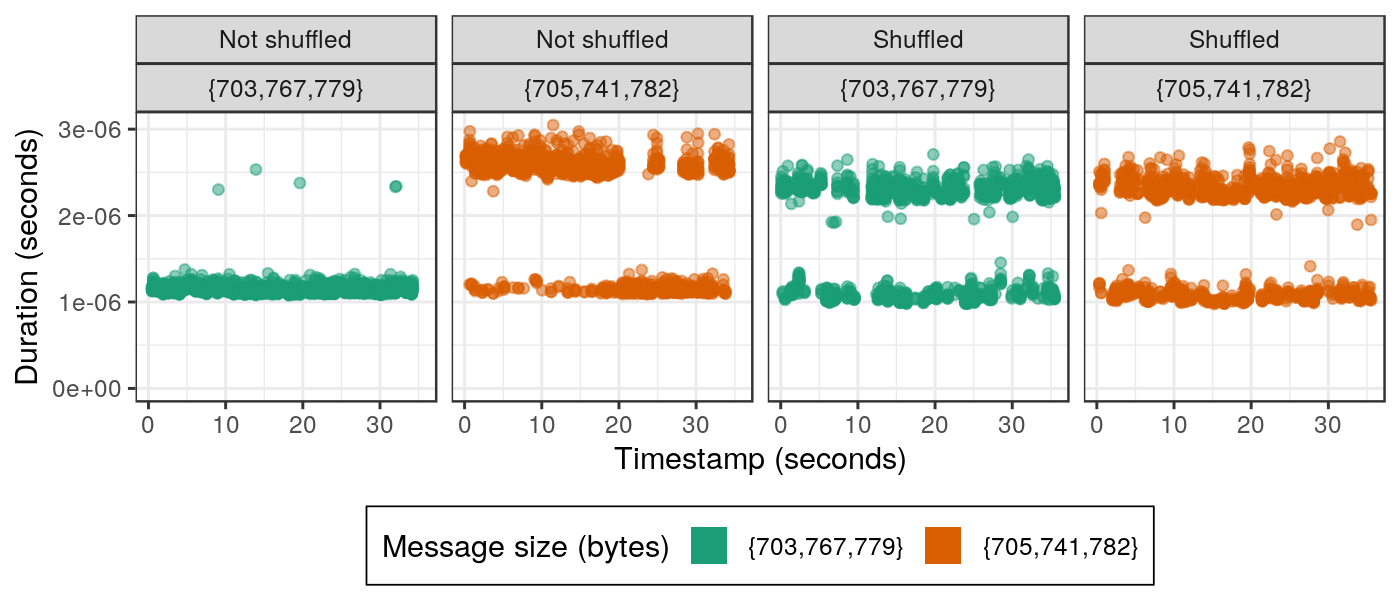
\includegraphics[width=\linewidth]{img/experiment/randomizing_order/evolution.png}
            \caption{Temporal evolution of the \recv durations for six different message sizes between \NSI{700}{\byte}
            and \NSI{800}{\byte}. A temporal pattern can be observed. Durations truncated to \NSI{4}{\micro\second} for
            a better readability.}%
            \label{fig:randomizing_order:evolution}
        \end{figure}

        Another view of the non-shuffled experiment is presented in Figure~\ref{fig:randomizing_order:evolution_rug}.
        Now all the calls with a size lower than \NSI{1}{\kilo\byte} are shown, but only a small fraction of the whole
        experiment is displayed. The calls to \recv can be divided into two groups depending on their durations, lower
        (in green) or greater (in orange) than \NSI{1.7}{\micro\second}. The rug plot on the top of the figure
        highlights the position in time of each of these \recv calls. Although there are slow and fast calls uniformly
        distributed during this time window, there appears to be some clusters where nearly all the calls are of the
        same kind.

        \begin{figure}[htpb]
            \centering
            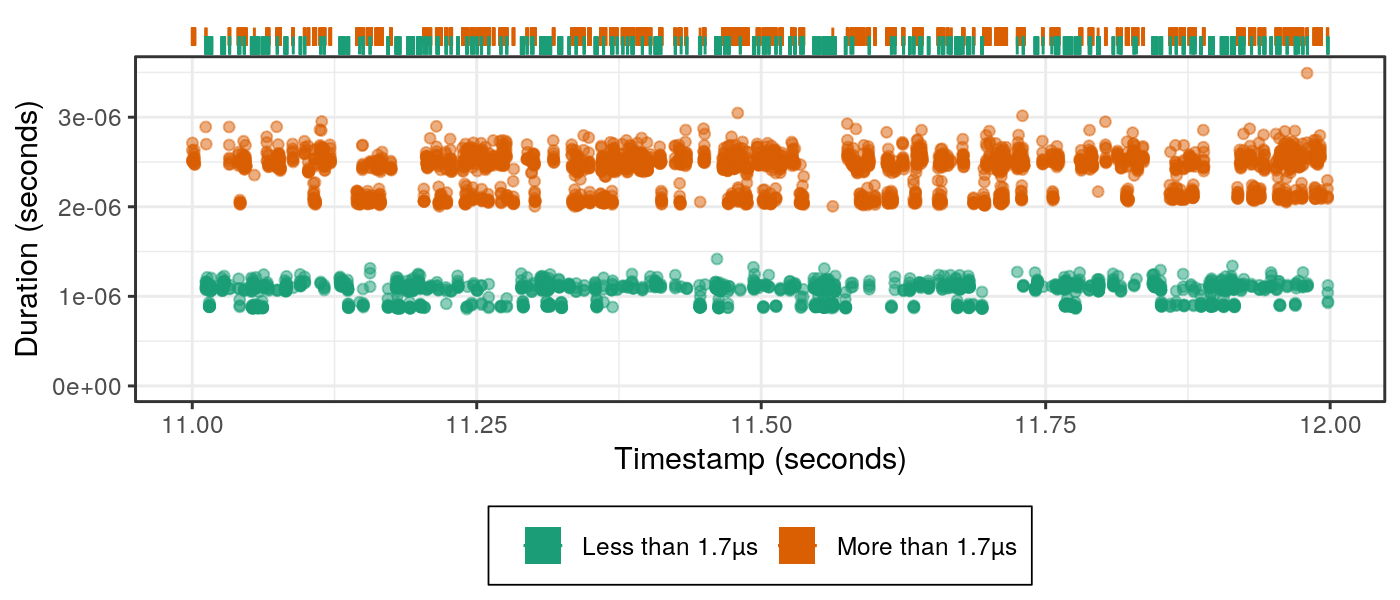
\includegraphics[width=\linewidth]{img/experiment/randomizing_order/evolution_rug.png}
            \caption{Temporal evolution of the \recv durations for all the sizes between \NSI{1}{\byte} and
            \NSI{1}{\kilo\byte} during a \NSI{0.2}{\second} time window of the non-shuffled experiment. Another temporal
            pattern can be observed.  Durations truncated to \NSI{4}{\micro\second} for a better readability.}%
            \label{fig:randomizing_order:evolution_rug}
        \end{figure}

        A possible explanation for such a temporal pattern could be an external perturbation that happens at a regular
        interval. Since we are measuring very small durations, the culprit would be a short but frequent noise (\eg a
        system daemon). This is very well explained by Petrini~\etal\cite{Petrini_2003}:
        \begin{quote}
            Substantial performance loss occurs when an application resonates with system noise: high-frequency,
            fine-grained noise affects only fine-grained applications; low-frequency, coarse-grained noise affects only
            coarse-grained applications.
        \end{quote}

        A similar temporal pattern can be observed in the shuffled experiment. However, since the order of the sizes is
        completely random, it affects them all equally.

        Later on, we went a step further in improving the methodology of this experiment by also randomizing the outer
        loop, \ie the measures are now shuffled, there are \emph{pingpong} measures between \emph{isend} and \emph{recv}
        measures and vice-versa. This change did not bring any noticeable effect on our observations.

        The experiments described in this section were performed in 2018. Two years later, we were unable to replicate
        this phenomenon, despite using the same MPI implementation and an identical cluster: the averaged data has a
        single mode, even in the non-shuffled case. We cannot state with certainty the reason this behavior disappeared,
        it could be due to a change in our calibration program, or on the platform itself. This motivates the
        implementation of performance non-regression tests, as discussed in Chapter~\ref{chapter:experiment:tests}.

    \section{Randomizing the sizes}%
    \label{sec:randomizing_sizes}
        %% TODO
        %% - Randomization de l'ordre des XPs HPL aussi mais pas de problème notable.
        %% - Les performances de MPI_Send,Recv dépendent de l'ordre du fichier d'expérience
        %%   (bon mélange des tailles ou non).
        %% - Les performances de dgemm dépendent de l'échantillonnage et de
        %%   l'échantillon (tests de non régression)
        %% - Les performances de dgemm dépendent de K (attendu), mais il y a un effet
        %%   mémoire (plus inattendu). Pour certains cas, souhaitable de calibrer à K
        %%   fixé. Dans ce cas là, isoler l'expérience du reste, ne pas essayer de mélanger
        %%   avec d'autres K.
        The calibration measures for the \dgemm function are done with a random sequence of tuples, as discussed in
        Section~\ref{sub:parameter_space:dgemm}. This sequence is properly shuffled, so we eliminated the possible
        experimental bias discussed in Section~\ref{sec:randomizing_order}. In this section, we will approach two
        difficulties that were encountered with the sizes themselves (as opposed to the order of the sequence).

        \subsection{Effect of the experiment file}%
        \label{sub:effect_experiment_file}

            Through the numerous \dgemm calibrations that were performed, we eventually realized that the set of sizes
            used for the experiment had a significant effect on the statistical model obtained with these measures. To
            demonstrate this, we have generated three different experiment files using exactly the same generation
            method described previously. These three experiments, named \texttt{A}, \texttt{B} and \texttt{C}, were
            repeated several dozen of times during a week-end in a random order. They have been carried on 8 different
            nodes of the dahu cluster, for a total of 16 different processors, the results are extremely similar for all
            of them.

            The average \dgemm performance observed in each experiment is reported in
            Figure~\ref{fig:randomizing_sizes:expfile:average_perf}. Some performance variability can be observed, the
            most efficient runs are approximately \NSI{3}{\percent} faster than the least efficient ones. A large
            fraction of this variability appears to be significantly caused by the experiment file, since all the runs
            made with file \texttt{C} have an higher performance than those made with file \texttt{B}, which are
            themselves more efficient than those made with file \texttt{A}. Thanks to the proper randomization of the
            experiments, we can rule out any temporal bias.

            \begin{figure}[htpb]
                \centering
                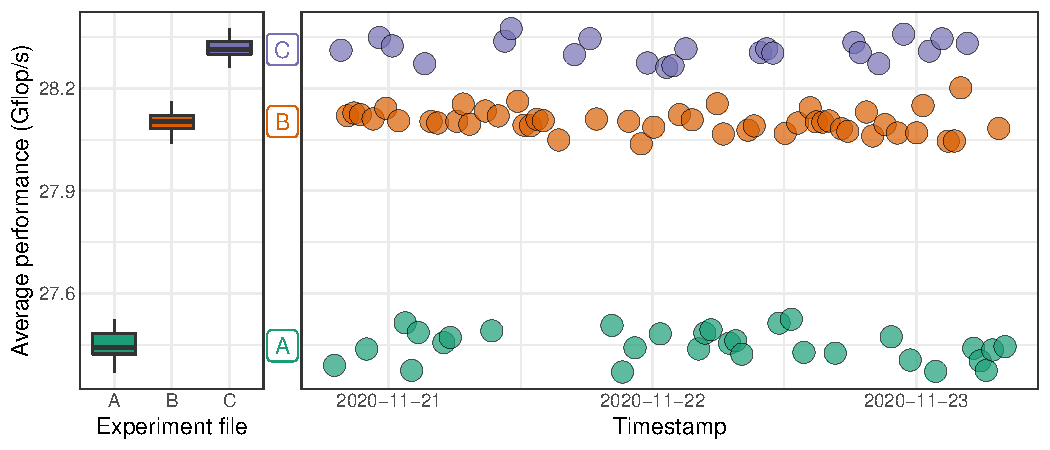
\includegraphics[width=\linewidth]{img/experiment/randomizing_sizes/expfile/average_performance.pdf}
                \caption{Average performance observed on CPU 1 of dahu-5, each point represents one experiment. A
                significant part of the variability is due to the choice of the experiment file.}%
                \label{fig:randomizing_sizes:expfile:average_perf}
            \end{figure}

            The effective performance is not the only aggregated metric affected by the choice of the experiment file.
            The distributions of two regression coefficients are represented in
            Figure~\ref{fig:randomizing_sizes:expfile:average_distribution}, namely the coefficients corresponding to
            the products \(MNK\) and \(NK\) (the effect of the experiment file on the coefficients for \(MK\) and \(MN\)
            is extremely similar to \(NK\)). It appears here that the experiment file causing the highest performance
            gives the highest cubic coefficient and the lowest quadratic coefficients. In other words, this means that
            with this experiment file, a larger fraction of the \dgemm durations is explained by the cubic coefficient.

            \begin{figure}[htpb]
                \centering
                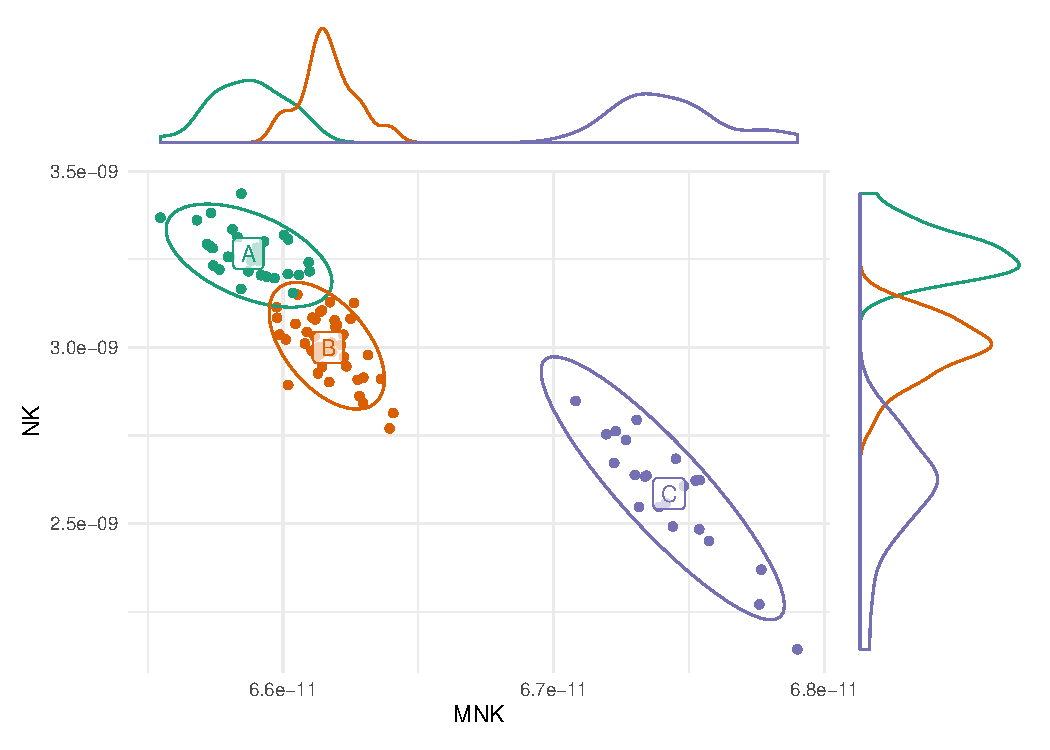
\includegraphics[width=\linewidth]{img/experiment/randomizing_sizes/expfile/average_distribution.pdf}
                \caption{Distribution of two of the regression parameters for CPU 1 of dahu-5, each point represents one
                experiment. The experiment file has a clear effect on the generated model}%
                \label{fig:randomizing_sizes:expfile:average_distribution}
            \end{figure}

            These observations suggest that experiments \texttt{A} and \texttt{B} may be less cache-friendly than
            experiment \texttt{C}, since in a matrix product the number of arithmetic operations grows cubically with
            the size of the input whereas the number of memory accesses grows quadratically.

            A non-aggregated view of the data is presented in Figure~\ref{fig:randomizing_sizes:expfile:raw_data}, each
            point represents one individual call to \dgemm. It appears that most of the calls in the three experiments
            have extremely similar durations for a given product \(MNK\). However, a small fraction of the \dgemm calls
            were significantly slower than the others with experiments \texttt{A} and \texttt{B}. All these calls have
            been made with a tall and skinny matrix, with \(K\geq3000\), which corroborates the hypothesis of a bad
            cache utilization.

            \begin{figure}[htpb]
                \centering
                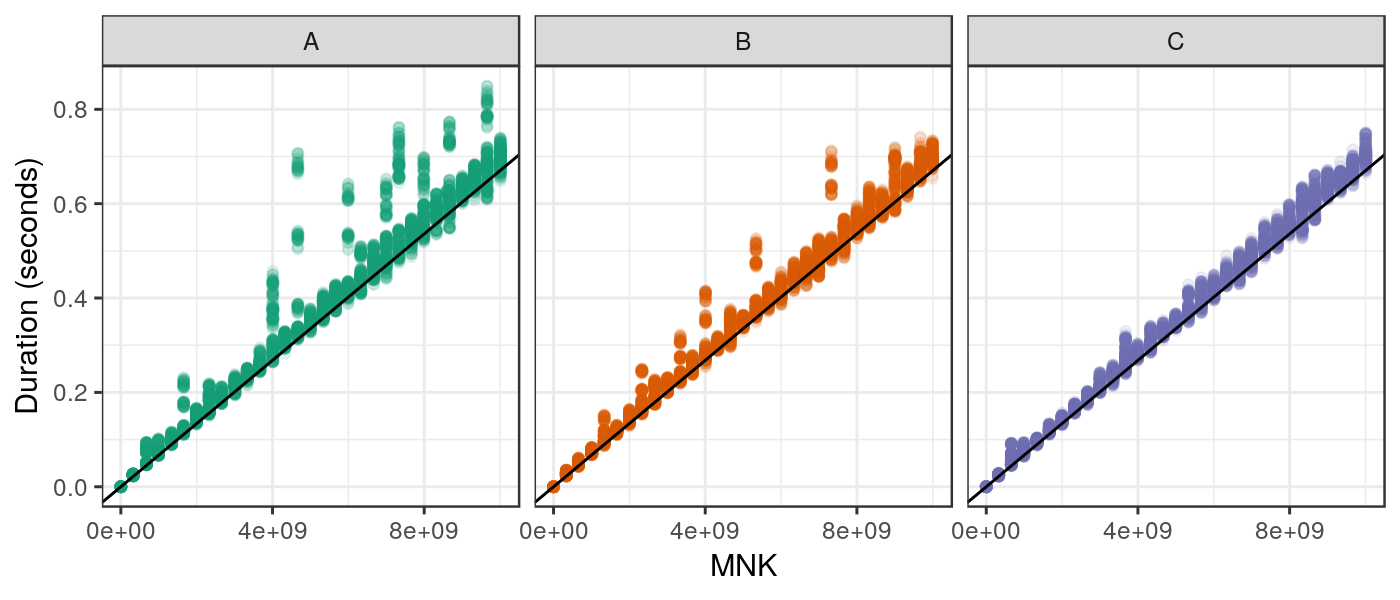
\includegraphics[width=\linewidth]{img/experiment/randomizing_sizes/expfile/raw_data.png}
                \caption{Durations of individual \dgemm calls for CPU 1 of dahu-5.
                Several calls have significantly longer durations than others. Identical black line on the three plots,
                with slope \Num{6.7e-11}.}%
                \label{fig:randomizing_sizes:expfile:raw_data}
            \end{figure}

            A final argument towards this hypothesis is presented with
            Figure~\ref{fig:randomizing_sizes:expfile:average_power}, the average DRAM power consumption during each run
            is presented. Similarly to Figure~\ref{fig:randomizing_sizes:expfile:average_perf}, there is a clear
            difference between the three experiments that cannot be explained by any temporal perturbation. Experiment
            \texttt{C}, which was the fastest, has the smallest DRAM power consumption. This suggests that the memory
            was used less intensively with this experiment, \ie there was a better cache utilization.

            \begin{figure}[htpb]
                \centering
                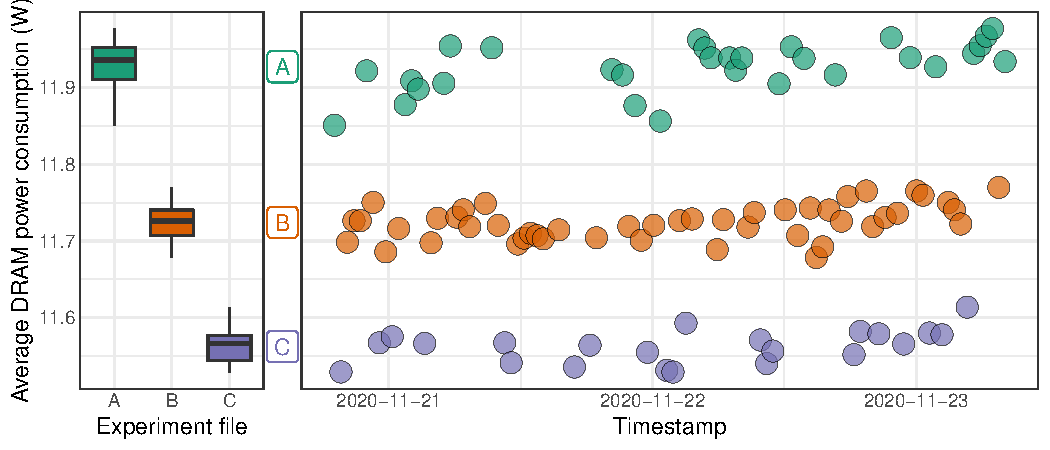
\includegraphics[width=\linewidth]{img/experiment/randomizing_sizes/expfile/average_power.pdf}
                \caption{Average DRAM power consumption observed on CPU 1 of dahu-5, each point represents one
                experiment.}%
                \label{fig:randomizing_sizes:expfile:average_power}
            \end{figure}

            In this section, we compared several \dgemm experiments performed with three sets of sizes. These sets have
            been generated according to the same statistical distribution, yet they lead to significantly different
            \dgemm models. We would like to stress that this discrepancy of the resulting models is due to a difference
            in the experimental conditions and not (only) to a statistical artifact. We proposed the hypothesis of a
            poor cache utilization, but other possibilities should not be dismissed, since this study was only
            observational, our hypothesis would need to be confirmed or refuted with a properly designed experimental
            study.

        \subsection{Effect of the experiment file generation method}%
        \label{sub:effect_experiment_file_generation_method}

            Section~\ref{sub:effect_experiment_file} has shown that the experiment file had a significant impact on the
            experimental conditions which affected the resulting statistical model. We generated three different
            sequence of sizes using the \emph{uniform product} method and performed several runs with each of these
            sequences.

            Now, we investigate briefly the effect of the generation method itself. We compare the \emph{independent
            sizes} and the \emph{uniform product} methods described in Section~\ref{sec:parameter_space}. For each of
            these methods, we generated several experiment files and performed one run with each of these files.

            Although there is a large variability, which is due to the use of several experiment files, it appears that
            the two generation methods lead to significantly different experimental conditions, as shown by
            Figure~\ref{fig:randomizing_sizes:expfile:method}. With the \emph{uniform product} method, \dgemm average
            performance is higher and the DRAM power consumption is lower.

            \begin{figure}[htpb]
                \centering
                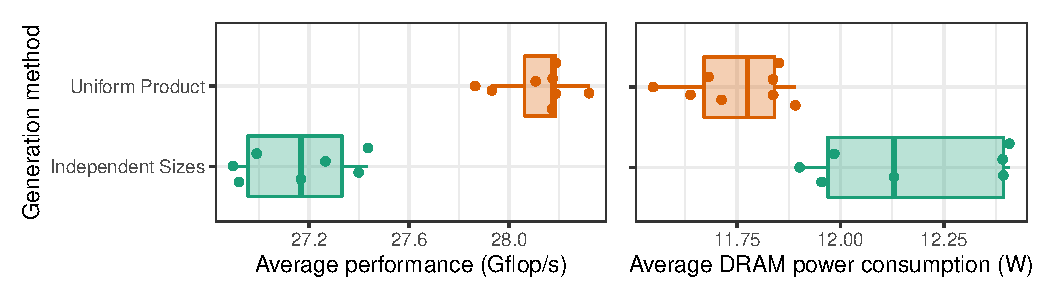
\includegraphics[width=\linewidth]{img/experiment/randomizing_sizes/method/average.pdf}
                \caption{Average \dgemm performance and power consumption observed on CPU 1 of dahu-5, each point
                represents one experiment.}%
                \label{fig:randomizing_sizes:expfile:method}
            \end{figure}


        \subsection{Effect of calibrating with a fixed size}%
        \label{sub:fixed_size}

            In the experiments described in Section~\ref{sub:effect_experiment_file} and
            Section~\ref{sub:effect_experiment_file_generation_method}, the three \dgemm parameters \(M\), \(N\) and
            \(K\) can take arbitrary values, to avoid any bias. One of the main reasons we make such measures is to
            generate a statistical model of \dgemm durations for simulating HPL. For this model to be faithful, the
            experimental conditions of our measures must be as realistic as possible to what happens during HPL
            execution. However, nearly all the \dgemm calls performed in HPL use the same value for the parameter \(K\),
            equal to HPL block size (\ie the parameter \texttt{NB}). For this reason, biasing the calibrations by using
            a fixed value for \(K\) could help to improve the simulation accuracy. This section investigates the
            question. We have generated five sets of experiment files:
            \begin{description}
                \item[Random] This is the usual \emph{uniform product} generation procedure already discussed in
                    previous sections.
                \item[Fixed K] We modified the \emph{uniform product} procedure to have a constant value for \(K\). We
                    generated three sets of files, with \(K=128\), \(K=256\) and \(K=512\).
                \item[Several fixed K] We modified the \emph{uniform product} procedure to have the value of \(K\)
                    chosen randomly in \{128,256,512\}. This is equivalent to concatenating three files generated with
                    the \emph{fixed K} method and then shuffling the resulting file.
            \end{description}
            For each of the five experiment kinds, we have generated several dozen of experiment files. Then, we
            performed one experiment with each of these files in a random order during a week-end on two nodes of the
            dahu cluster for a total of four different processors. Again the results are similar for all of them, so we
            will focus on a single processor.

            Figure~\ref{fig:randomizing_sizes:expfile:fixing_K:performance} presents the observed \dgemm performance
            with the five experiments. We can observe that again, the generation method for the size sequence has a huge
            effect on the experiment. First, using a fixed value for \(K\) reduces very significantly the inter-run
            performance variability. The average performance is also greatly affected, it is the highest with \(K\)
            fixed to 128, the lowest with \(K\) fixed to 256 or 512 or with the random generation, and it is
            intermediate with \(K\) randomly sampled in \(\{128,256,512\}\).

            \begin{figure}[htpb]
                \centering
                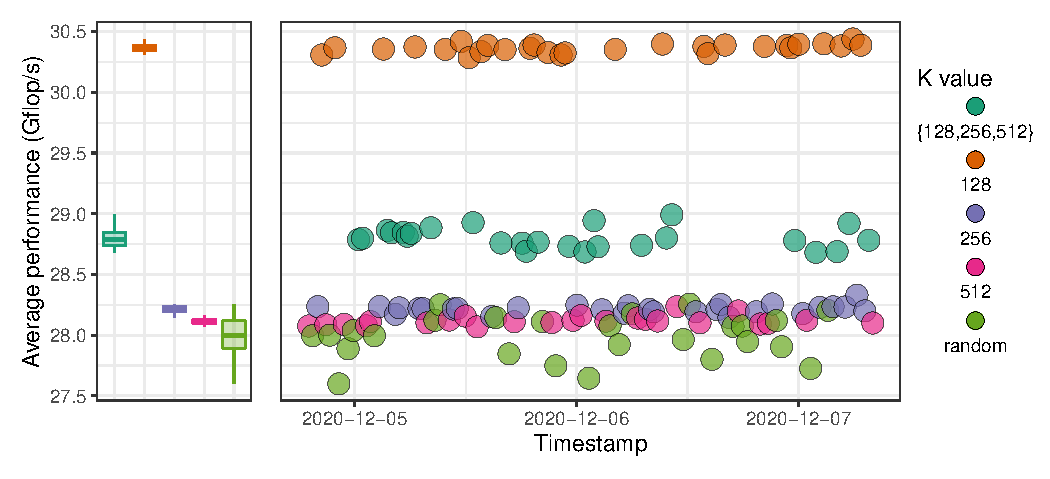
\includegraphics[width=1\linewidth]{img/experiment/randomizing_sizes/fixing_K/average_performance.pdf}
                \caption{Average \dgemm performance observed on CPU 1 of dahu-5, each point represents one experiment.}%
                \label{fig:randomizing_sizes:expfile:fixing_K:performance}
            \end{figure}

            The monitoring data collected during the experiments also reveal interesting differences. The average CPU
            frequency is reported in Figure~\ref{fig:randomizing_sizes:expfile:fixing_K:frequency}. It appears that the
            frequency is the highest with \(K=128\) and with the random experiment. It is significantly lower with \(K\)
            chosen randomly among the three sizes, and even lower with \(K=256\) and \(K=512\). It is interesting to
            note that there is a positive correlation between the frequency and \dgemm performance, but the random
            experiment is a clear exception as it leads to a relatively low performance and high frequency.

            \begin{figure}[htpb]
                \centering
                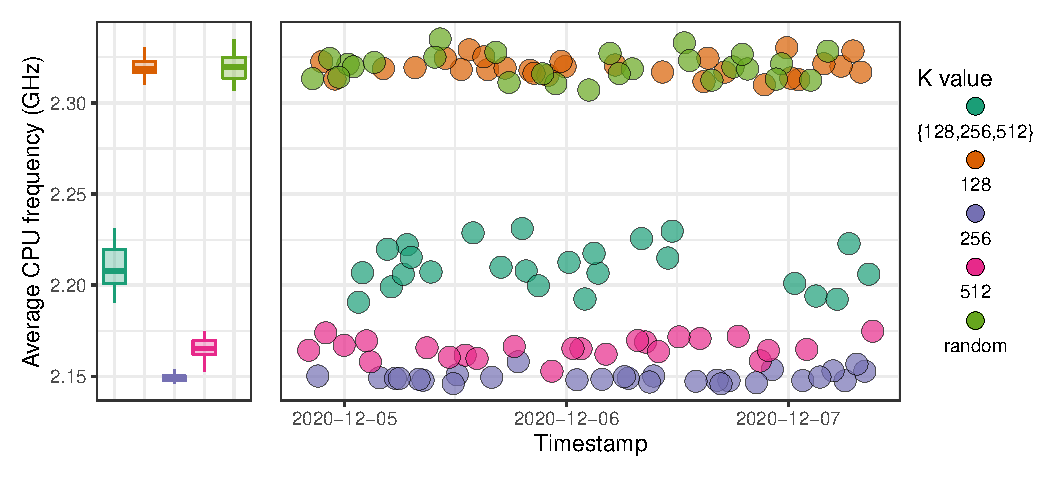
\includegraphics[width=1\linewidth]{img/experiment/randomizing_sizes/fixing_K/average_frequency.pdf}
                \caption{Average CPU frequency, observed on CPU 1 of dahu-5, each point represents one experiment.}%
                \label{fig:randomizing_sizes:expfile:fixing_K:frequency}
            \end{figure}

            The average CPU power consumption, presented in
            Figure~\ref{fig:randomizing_sizes:expfile:fixing_K:power_CPU}, is particularly peculiar. The random
            experiment has a power consumption significantly lower and more variable than the four other experiments
            that are all extremely stable, with nearly no inter-run variability. This observation is very
            counter-intuitive, since the CPU power consumption is in general proportional to the CPU
            frequency~\cite{heinrich:hal-01523608}.  This only happens on the CPU 1 of the two nodes we tested, the
            power consumption of the CPU 0 is extremely stable and similar for the five experiment kinds.

            \begin{figure}[htpb]
                \centering
                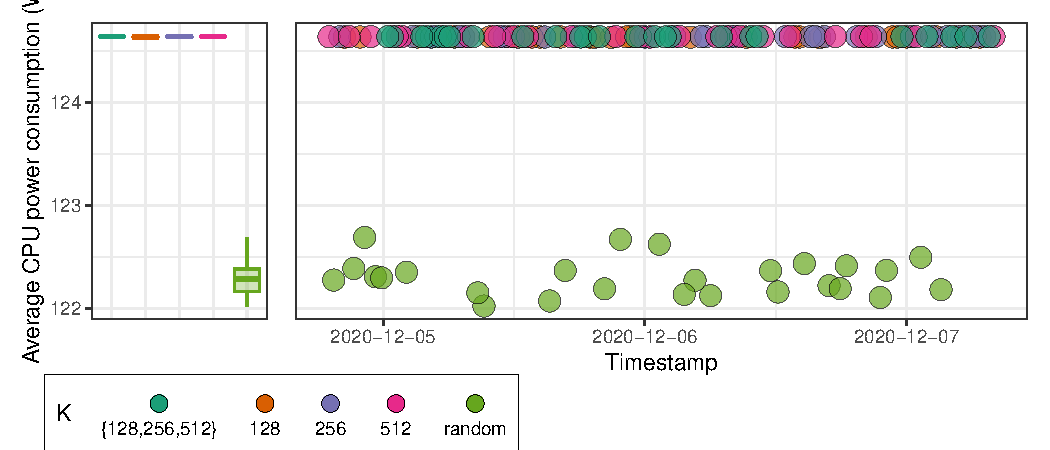
\includegraphics[width=1\linewidth]{img/experiment/randomizing_sizes/fixing_K/average_power_CPU.pdf}
                \caption{Average CPU power consumption, observed on CPU 1 of dahu-5, each point represents one experiment.}%
                \label{fig:randomizing_sizes:expfile:fixing_K:power_CPU}
            \end{figure}

            The five experiments exhibit very different average DRAM power consumption, as depicted in
            Figure~\ref{fig:randomizing_sizes:expfile:fixing_K:power_DRAM}. The experiment with \(K=128\) is the most
            energy-hungry, followed by the experiment with \(K\in\{128,256,512\}\), then the experiments with a random
            \(K\), \(K=256\) and \(K=512\). It is interesting to note that the experiment with the highest DRAM power
            consumption is also the one with the highest average \dgemm performance, which is the opposite of what was
            observed in Section~\ref{sub:effect_experiment_file}.
            \begin{figure}[htpb]
                \centering
                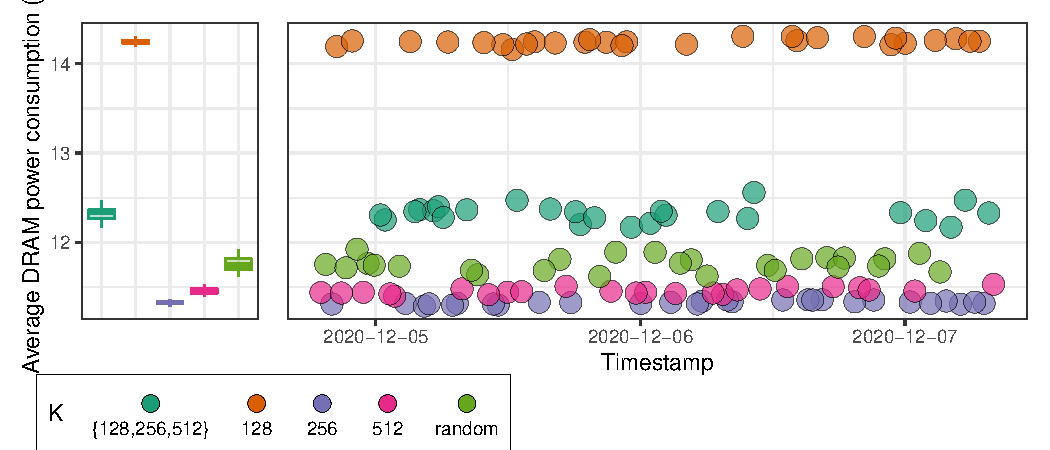
\includegraphics[width=1\linewidth]{img/experiment/randomizing_sizes/fixing_K/average_power_DRAM.pdf}
                \caption{Average DRAM power consumption, observed on CPU 1 of dahu-5, each point represents one experiment.}%
                \label{fig:randomizing_sizes:expfile:fixing_K:power_DRAM}
            \end{figure}

            Finally, the performance of individual \dgemm calls are presented in
            Figure~\ref{fig:randomizing_sizes:expfile:fixing_K:raw_data}. We made the observation earlier that there was
            much less inter-run variability when the value of \(K\) was fixed. This plot shows that there is also
            significantly less intra-run variability. Furthermore, we can compare the performance of \dgemm for a given
            value of \(K\). With \(K=128\), the performance is higher in the experiment where all the calls are done
            with \(K=128\) than in the experiment with \(K\in\{128,256,512\}\). With the two other values, \(K=256\) and
            \(K=512\), this is the opposite, the performance is higher in the mixed experiment than in the experiment
            with only one \(K\) value. This shows that the durations of individual \dgemm calls are not independent, one
            call can be faster or slower depending on the calls previously made.
            \begin{figure}[htpb]
                \centering
                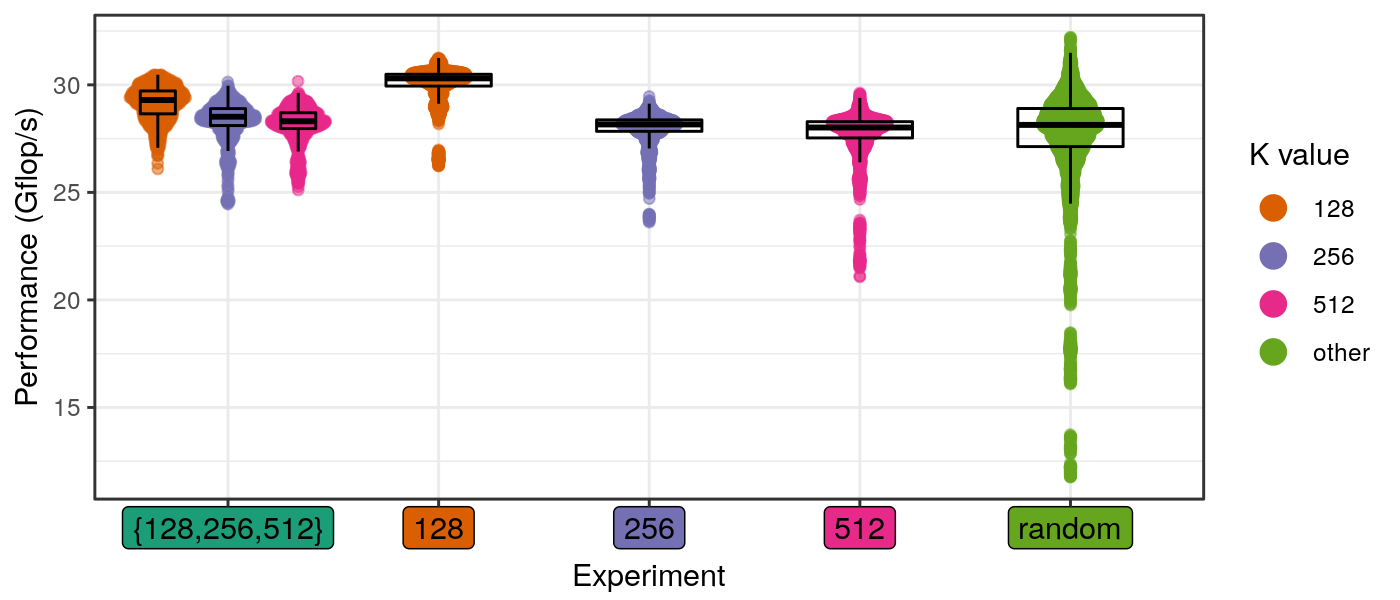
\includegraphics[width=1\linewidth]{img/experiment/randomizing_sizes/fixing_K/raw_data.png}
                \caption{Durations of individual \dgemm calls for CPU 1 of dahu-5.}%
                \label{fig:randomizing_sizes:expfile:fixing_K:raw_data}
            \end{figure}

            In this section, we demonstrated once again that the sampling method has an important effect on the measured
            performance. This will affect any statistical model we could build using the measured data, not because of a
            statistical bias, but because of an experimental bias. Such a bias might be desirable, for instance it
            should help improve the prediction accuracy of our HPL simulations. It comes at a price though, since we
            need to perform a new \dgemm calibration if we want to simulate HPL with another block size.

    \section{Randomizing the data}%
    \label{sec:randomizing_data}
        %% TODO
        %% - Les performances de dgemm dépendent du contenu de la matrice (random ou
        %%   constant par exemple). Ça serait causé par des bit flips dans le CPU qui
        %%   engendre une plus grande consommation (réutiliser le rapport).
        The work presented in this section has been published as a technical report~\cite{cornebize:bitflips}. The
        content of this section is therefore a near-verbatim copy of this report.

        This experiment comes, yet again, from an unfortunate phenomenon we stumbled upon when calibrating the platform
        for our simulations. Our predictions were wrong, so we investigated a bit and we noticed a significant mismatch
        between the durations measured with our calibration code and the durations observed in HPL. We found out that,
        the performance of the \dgemm function depends on the content of the matrix, which was unexpected.

        \subsection{Randomization of the matrix initialization}
        \label{sub:randomization_matrix_initialization}
            The three matrices are allocated once at the start of the program as a buffer of size \(N^2\) with
            \(N=2,048\). Then, their content is initialized in three different ways, depending on the experiment:
            \begin{enumerate}
                \item All the elements of the matrices are equal to some constant. We have tested with three different
                    values: 0, 0.987 and 1.
                \item The elements of the matrices are made of an increasing sequence in the interval \([0, 1]\). More
                    precisely, \texttt{mat[i] = i/(N\textasciicircum{}2-1)} for i in \([0, N^2-1]\).
                \item Each element of the matrix is randomly and uniformly sampled in the interval \([0, 1]\).
            \end{enumerate}

        Figure~\ref{fig:exp:bit-flips:method-perf} shows the evolution of the \dgemm durations during the experiment.
        A clear temporal patterns can be distinguished, the performance is oscillating.  Furthermore, several layers can
        be seen, the durations of \dgemm are the highest when the matrices are initialized randomly and the
        lowest when they are initialized with a constant value. The sequential initialization is in between.

        \begin{figure}[htbp]
            \centering
            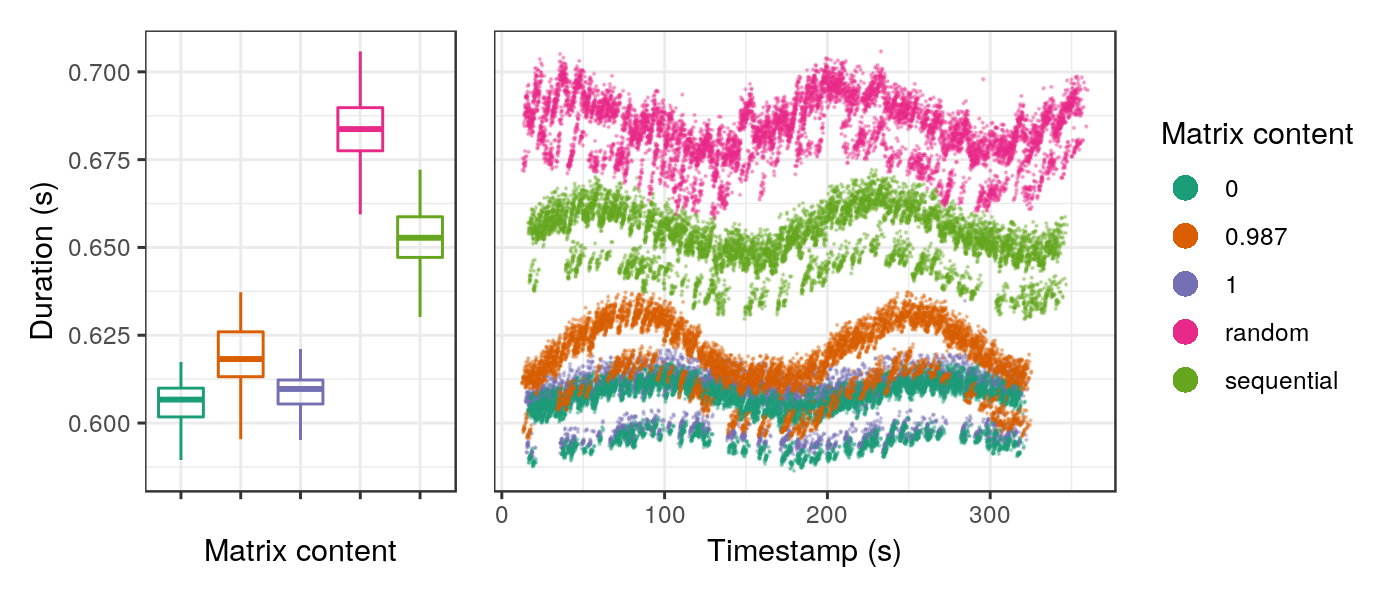
\includegraphics[width=\linewidth]{img/experiment/bit-flips/generation_method_perf.png}
            \caption{\label{fig:exp:bit-flips:method-perf}
            \dgemm durations are lower with constant values in the matrices}
        \end{figure}

        Such an observation was unforeseen. The function \dgemm implements the usual matrix product with cubic
        complexity. The control flow of the function does not depend on the matrix content, so we did not expect its
        duration to be data-dependent.

        The observations we have made on \dgemm performance can be explained by
        Figure~\ref{fig:exp:bit-flips:method-freq} which shows the evolution and the distribution of the core
        frequencies during the experiment. There is a clear correlation between the frequencies and \dgemm
        performance: the random initialization produces lower frequencies whereas the constant initialization gives
        higher frequencies. A similar temporal patterns can also be distinguished with clear oscillations.

        \begin{figure}[htbp]
            \centering
            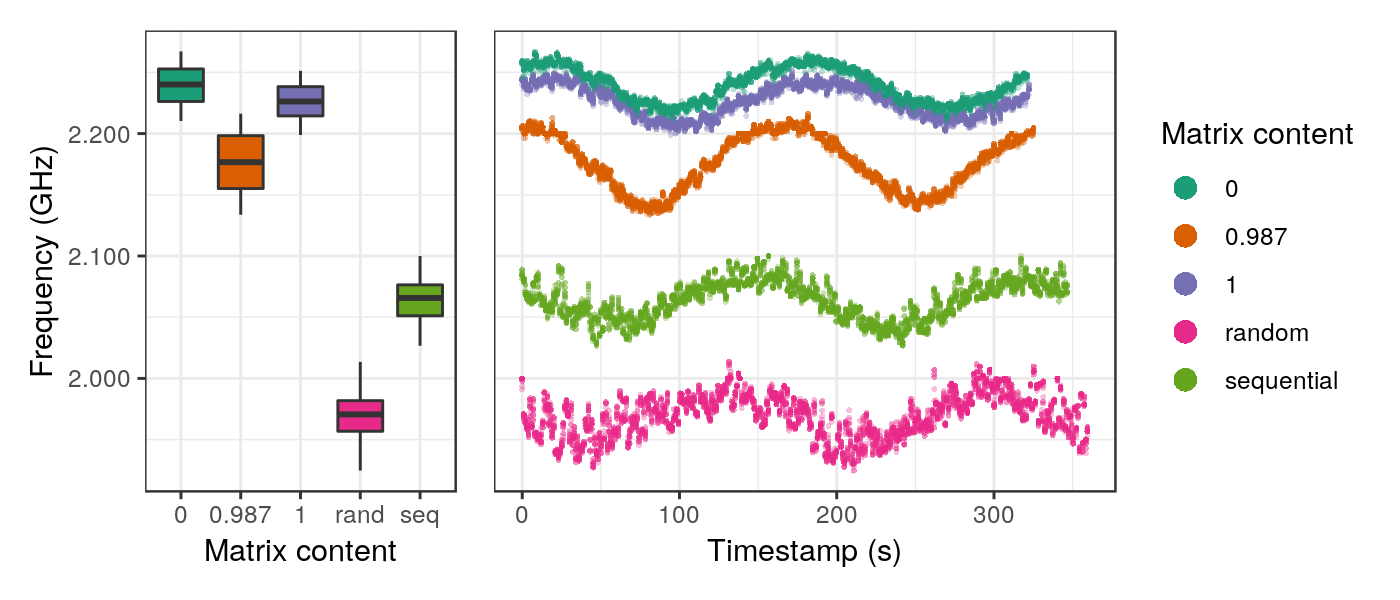
\includegraphics[width=\linewidth]{img/experiment/bit-flips/generation_method_freq.png}
            \caption{\label{fig:exp:bit-flips:method-freq}
            Core frequencies are higher with constant values in the matrices}
        \end{figure}

        This experiment has been repeated on other Grid'5000 clusters, each time on at least four distinct nodes.
        Table~\ref{tab:bit-flips} gives a summary of our observations. Five other clusters show a similar behavior, the
        performance of \dgemm is higher when the matrices are generated with a constant value. However, for five
        other clusters, this phenomenon could not be observed, the matrix content had no impact on the performance.
        %% TODO run this experiment on other Grid'5000 clusters, just to extend a bit the table of the clusters we tested it on.
        %% I have at least two clusters in mind:
        %% - pyxis (ARM processors)
        %% - troll (newest generation of Intel processors, Cascade Lake)

        \begin{table}[htbp]
            \caption{\label{tab:bit-flips}
            Observation of the  performance anomaly on Grid'5000 clusters}
            \centering
            \begin{tabular}{lllll}
                \toprule
                Cluster & CPU & Generation & Release date & Anomaly\\
                \midrule
                nova & Intel Xeon E5-2620 v4 & Broadwell & Q1'12 & no\\
                taurus & Intel Xeon E5-2630 & Sandy Bridge & Q1'12 & no\\
                ecotype & Intel Xeon E5-2630L v4 & Broadwell & Q1'12 &yes\\
                paranoia & Intel Xeon E5-2660 v2 & Ivy Bridge & Q3'13 & no\\
                parasilo & Intel Xeon E5-2630 v3 & Haswell & Q3'14 & yes\\
                chiclet & AMD EPYC 7301 & - & Q2'17 & no\\
                dahu & Intel Xeon Gold 6130 & Skylake & Q3'17 & yes\\
                yeti & Intel Xeon Gold 6130 & Skylake & Q3'17 &yes\\
                pyxis & ARM ThunderX2 99xx & - & Q2'18 & no\\
                gros & Intel Xeon Gold 5220 & Cascade Lake & Q2'19 & yes\\
                troll & Intel Xeon Gold 5218 & Cascade Lake & Q2'19 & yes\\
                \bottomrule
            \end{tabular}
        \end{table}

        \subsection{Hypotheses}
            %% TODO add the hypothesis on subnormal numbers.
            Several hypotheses were discussed to explain this unexpected phenomenon.

            There could be a small cache  on the floating point unit of the cores to memorize the results of frequent
            operations. This could explain why the durations were higher when the matrices were initialized randomly,
            but this does not explain why the sequential initialization is in between.

            This could be due to kernel same page merging (KSM), a mechanism that allows the kernel to share identical
            memory pages between different processes. Again, this would explain the difference between the random
            initialization and the constant one, but not why the sequential initialization gives intermediate
            performance.

            A last hypothesis is the power consumption of the cores. Each state change of the electronic gates of the
            CPU costs an energy overhead. In the case of the constant initialization, the registers will change less
            often during the execution of \dgemm, in comparison with the random initialization. Thus, with the
            constant initialization, the processor cores would be able to maintain a higher frequency while respecting
            the thermal design power (TDP), with the random initialization the frequency would be throttled more
            aggressively and thus the performance would be lower.
            As for the sequential initialization, we can imagine that we have a locality effect: nearby elements of the
            matrices will have more bits in common, this would causes less bit flips than the random initialization but
            more bit flips than the constant initialization and thus an intermediate performance.

        \subsection{Testing the bit-flip hypothesis}
            To test the hypothesis that the lower frequencies are caused by more frequent bit flips in the processor,
            the matrix initialization has been changed. Now, each element of the matrix is randomly and uniformly
            sampled in the interval \([0,1]\). Then a bit mask is applied on the lower order bits of their mantissa. As
            a result, all the elements of the matrices have some bits in common. This method is illustrated in
            Figure~\ref{fig:exp:bit-flips:mask_illustration}, the mantissa of the matrix elements (in blue) is at first
            completely random, then we apply a mask so that the right-most bits (in green) become
            deterministic\footnote{Image adapted from
            \url{https://en.wikipedia.org/wiki/Double-precision_floating-point_format}}.  Several mask sizes have been
            tested, from 0 (the elements are left unchanged) to 53 (the mantissa becomes completely deterministic, all
            the elements are equal).
            \begin{figure}[htpb]
                \begin{center}
                    \includesvg[width=\linewidth]{img/experiment/bit-flips/float.svg}
                    \vspace{-0.2cm}

                    
\begin{tikzpicture}
                        \draw[->, line width=1mm] (0,0) -- (0,-1);
                    \end{tikzpicture}

                    \vspace{-0.2cm}
                    \includesvg[width=\linewidth]{img/experiment/bit-flips/float_mask.svg}
                \end{center}
                \caption{Illustrating the effect of applying a mask on the random part of the matrix
                elements\label{fig:exp:bit-flips:mask_illustration}}
            \end{figure}

            The evolution and the distribution of the \dgemm durations is plotted in
            Figure~\ref{fig:exp:bit-flips:mask-perf}. Their is a very clear correlation between the mask size and the
            performance: the larger the mask, the lower the duration. Similarly to the previous experiment, some
            temporal patterns can also be distinguished.

            \begin{figure}[htbp]
                \centering
                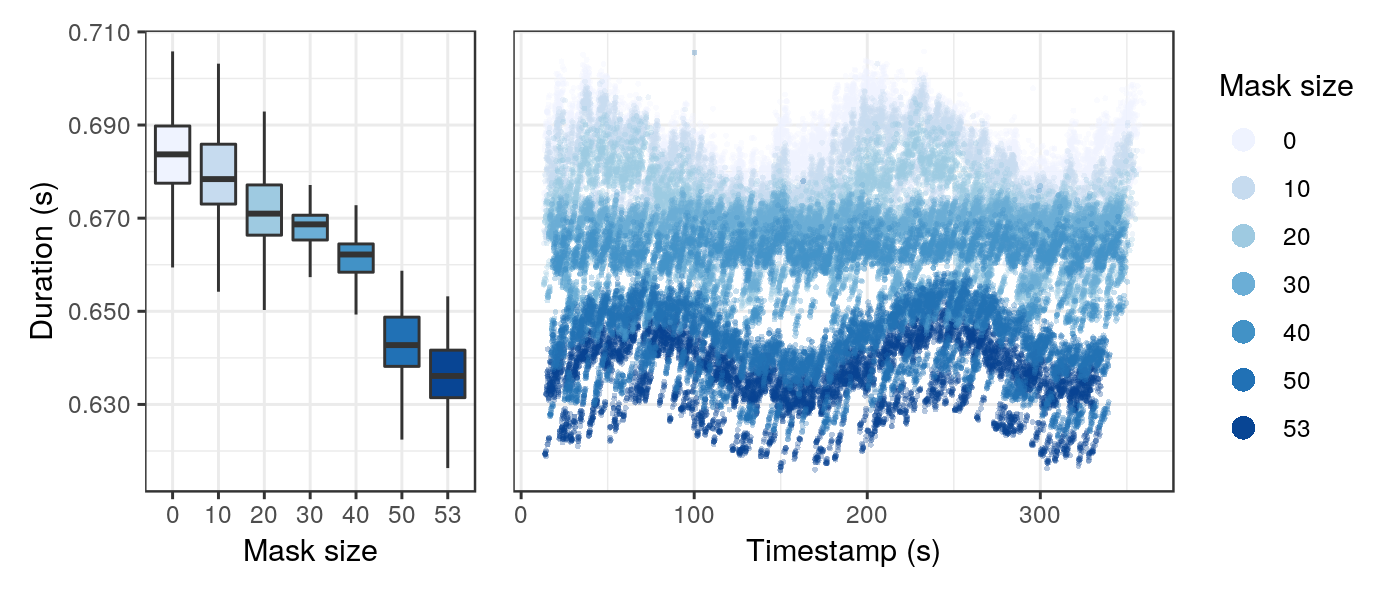
\includegraphics[width=\linewidth]{img/experiment/bit-flips/mask_size_perf.png}
                \caption{\label{fig:exp:bit-flips:mask-perf}
                \dgemm durations are lower with larger bit masks}
            \end{figure}

            This correlation with the mask size can also be seen with the frequencies in
            Figure~\ref{fig:exp:bit-flips:mask-freq}: larger masks lead to higher frequencies.

            \begin{figure}[htbp]
                \centering
                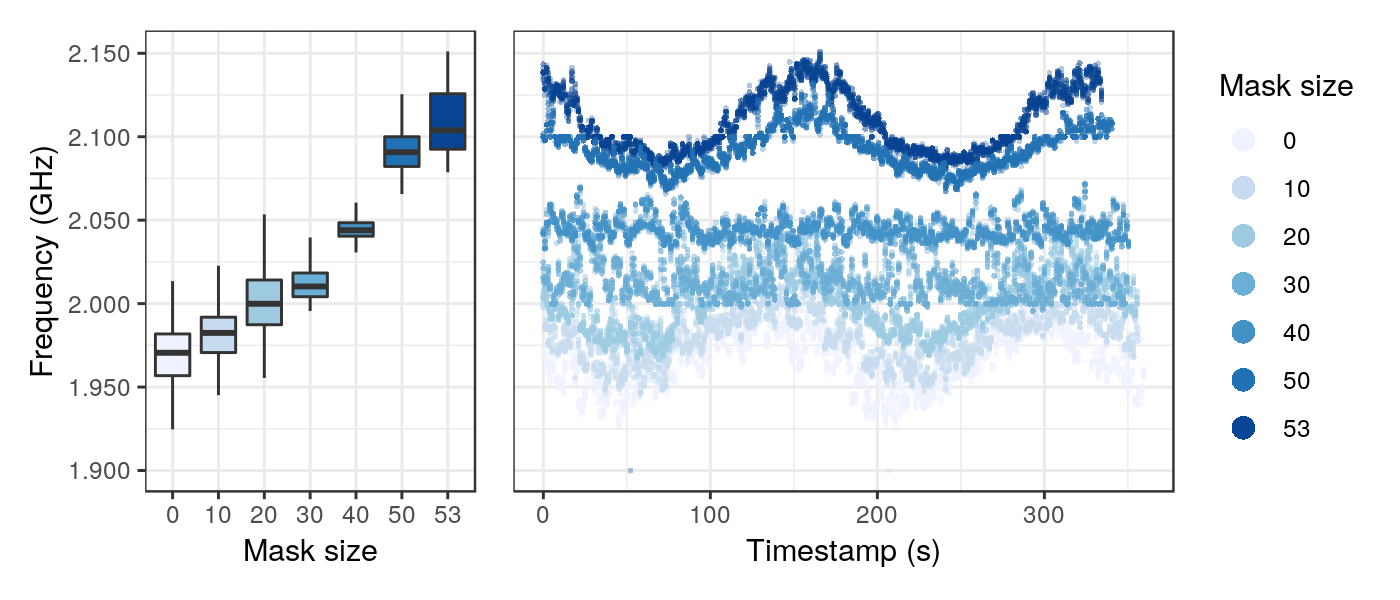
\includegraphics[width=\linewidth]{img/experiment/bit-flips/mask_size_freq.png}
                \caption{\label{fig:exp:bit-flips:mask-freq}
                Core frequencies are higher with larger bit masks}
            \end{figure}

            This experiment has been repeated on two other Grid'5000 clusters, ecotype and gros. For both of them, the
            same observations could be made, a clear correlation between the mask size, the frequencies and the
            performance.

        \subsection{Conclusion}
            We have shown that the performance of the \dgemm function is data-dependent. The best explanation we
            have for this counter-intuitive fact is an energy cost overhead caused by bit flips inside the processor.
            To respect its energy budget, the CPU has to throttle more aggressively its frequency when the matrices
            content is more diverse and thus more energy consuming.
            This theory has been corroborated by a controlled experiment where the elements of the matrices are
            initialized semi-randomly: they all share an identical bit suffix.

            To strengthen this claim further, the next steps will be to perform a similar experiment with another
            compiler, another BLAS library and/or another computation kernel. We also need to understand why some
            processors are subject to this phenomenon and some others are not.

            We warmly thank our colleagues that helped us to find hypotheses for this performance anomaly. In
            particular, Guillaume Huard suggested that the performance anomaly may be caused by the bit flips in the
            processor.

        \subsection{Related work}%
            M. La{\ss}, C. Plessl and R. Schade (Paderborn Center for Parallel Computing) made independently similar
            observations (personal communications on 2020/09/24 and 2020/11/11). Their findings is summarized here:
            \begin{itemize}
                \item They observed that \dgemm performance depended on the content of the matrix. They also
                    made the hypothesis that it was caused by bit-flips. To test this hypothesis, they used the same
                    approach, they filled the matrices with random values with a mask applied to the lower-order bits.
                    They observed a correlation between the mask size and \dgemm performance, which is an
                    argument in favor of this hypothesis. This experiment was done using another \dgemm
                    implementation than us (Intel MKL) on an Intel Xeon Gold 6148 (Skylake-SP family) from a noctua
                    node\footnote{\url{https://pc2.uni-paderborn.de/hpc-services/available-systems/noctua/}}.
                \item They reproduced the same experiment on a FPGA (more precisely, a Bittware 520N PCIe accelerator
                    card, equipped with an Intel Stratix 10 GX 2800 FPGA). This time, the way the matrix was filled had
                    an effect on the power consumption and not the performance. This was expected since there is no DVFS
                    on FPGA.
                \item To see whether the effect was caused by the CPU arithmetic units or the cache, they adapted a
                    micro-benchmark\footnote{\url{https://github.com/pc2/Flops}} to perform multiplications with more or
                    less random data, using only the registers of the CPU. They did not observe any difference of
                    performance caused by the data, but they did observe a higher power consumption of \SI{5}{\percent}
                    with random data. This power consumption remained under the TDP even after the increase, so the CPU
                    frequency did not get throttled.
            \end{itemize}

            Sch{\"{o}}ne~\etal~\cite{DBLP:journals/corr/abs-1905-12468} observed a data-dependent power consumption with
            a Skylake-SP processor using AVX instructions. Note that in their experiment, the core frequency and the
            instruction rate were constant.

            Andr\'e~\etal~\cite{andre:hal-02401796} observed in one of their experiments that limiting the uncore
            frequency (\ie the frequency of the L3 cache and the memory controller) can increase the performance of HPL
            by about \SI{1.5}{\percent}. The reason is that HPL power consumption reaches TDP, so lowering the uncore
            frequency allows a higher power consumption of the cores and thus a higher frequency.

    \section{Beware of extrapolations}%
    \label{sec:beware_of_extrapolations}
        \todo{Should we remove this section? It seems pretty obvious and uninteresting...}
        %% TODO
        %% Le problème est survenu dans plusieurs cas de figure, notamment
        %% pour HPL avec des géométries très élongées.
        %% - Les prédictions pour dgemm n'étaient plus très bonnes. On extrapolait trop
        %%   loin, la calibration était faite avec M<=15000 et N<=15000 alors que pour de
        %%   telles géométries on avait parfois des tailles 10\times plus grandes (les
        %%   produits MNK avaient le même ordre de grandeur par contre).
        %% - Les prédictions pour les communications étaient également mauvaises, en
        %%   partie parce que l'on calibrait pour des messages jusqu'à 1MB et on
        %%   esssayait de prédire la durée de communications de 1GB.
        %% - Parler de notre tentative d'extrapolation de HPL sur (P,Q) ? Peut être plutôt en partie 1.
        In several occasions when working on Part~\ref{part:prediction}, we found that our predictions were inaccurate
        because of a wrong extrapolation. The measures made for instantiating the model were made with parameters that
        were very different to the ones needed when using these models in simulation. This happened at least twice, with
        the \dgemm function and with MPI communications.

        \begin{description}
            \item[Function \dgemm] The model used to be instantiated using the durations of \dgemm calls made with
                random arguments \(M,N\) and \(K\), as described in Section~\ref{sec:parameter_space}. The maximum value
                of these three parameters was \Num{15000}. However, when HPL is executed with very elongated
                geometries (\eg a very small \texttt{P} or a very small \texttt{Q}), it performs \dgemm calls with very
                elongated matrices. We observed in some experiments that \(M\) or \(N\) could take values as large as
                \Num{150000} while the two other parameters remained rather small. In these conditions, the durations of
                individual \dgemm calls are much more variable, while the average performance is slightly lower.
            \item[Functions \recv and \send] In the legacy script for calibrating MPI communications for Simgrid, the
                message size was sampled randomly, with a maximum size of \NSI{1}{\mega\byte}. However, similarly to the
                \dgemm calibration issue we had, some communications in HPL are much larger, up to \NSI{1}{\giga\byte}
                in our experiments. When increasing the maximal size, we found out that the network performance drops
                very significantly at some point.
        \end{description}

        These two examples can seem obvious after the fact. Yet, they show the difficulty of anticipating when the usage
        of a model will reaches its limits. In both cases, we had to instrument the HPL code to generate a trace and
        find that the parameters space used in the calibration was very different than the parameter space used during
        the execution. One way to limit the risk of missing such extrapolations would be to define explicitly in the
        model files the parameter ranges that were used for calibrating them. Then, during a simulation, we could raise
        a warning whenever a model is used outside of its parameter space.


    \section{Beware of experimental conditions}%
    \label{sec:beware_of_experimental_conditions}
        %% TODO
		%% - Chauffe des CPU avant au cas où. Brice et Kevin monitoraient la
		%%   température au fil de l'expérience et arrêtaient les mesures quand
		%%   c'était trop chaud.
		%% - Dans HPL, il semble que les calculs ralentissent beaucoup certaines
		%%   communications. Ce phénomène n'était initialement pas capturé par la
		%%   calibration puisque les mesures étaient faites sans aucun calculs à
		%%   côté.
        We already have demonstrated numerous times in previous sections that the experimental conditions are of utmost
        importance in this work, any change can have a significant effect on the measures, as harmless as it may seem.
        In this section, we give some details on an interaction between computations and MPI communications we observed
        while working on Part~\ref{part:prediction}.

        We compare four different scenarios for sending a message of \NSI{256}{\mebi\byte} with MPI. For each scenario,
        we performed two experiments, one where this communication happens locally and another one where it is done
        remotely. The result is presented in Figure~\ref{fig:experiment:experimental_conditions}.
        \begin{itemize}
            \item Scenario \texttt{idle}. Two MPI ranks perform a simple ping-pong with the aforementioned message. Each
                MPI rank is bound to one core (either two cores of the same node for the loopback communication, or two
                cores of distinct nodes in the remote case). All the other cores are kept idle.
            \item Scenario \dgemm. This one is identical to the scenario \texttt{idle}, except that all the cores not
                involved in the communication are performing \dgemm calls.
            \item Scenario \texttt{MPI\_Iprobe}. The communication pattern is more elaborated in this scenario. It uses
                two nodes, for a total of 64 cores. It repeats several times a sequence of 64 steps, where at step \(i\)
                the MPI rank \(i\) performs a ping-pong with the MPI rank \((i+1)\mod64\). This is similar to a ring
                broadcast, except that the ranks perform a two-way exchange instead of one-way. All the ranks waiting
                for an incoming communication are performing a busy waiting, looping on the result of the function
                \texttt{MPI\_Iprobe}.
            \item Scenario \texttt{MPI\_Iprobe} \& \dgemm. This scenario is identical to the \texttt{MPI\_Iprobe}
                scenario, except that every rank performs a call to function \dgemm between any call to function
                \texttt{MPI\_Iprobe}.
        \end{itemize}

        The two last scenarios can appear oddly twisted. The goal was, again, to implement a micro-benchmark that is as
        close as possible to what happens in the real application we tried to model, HPL in this case.

        \begin{figure}[htpb]
            \centering
            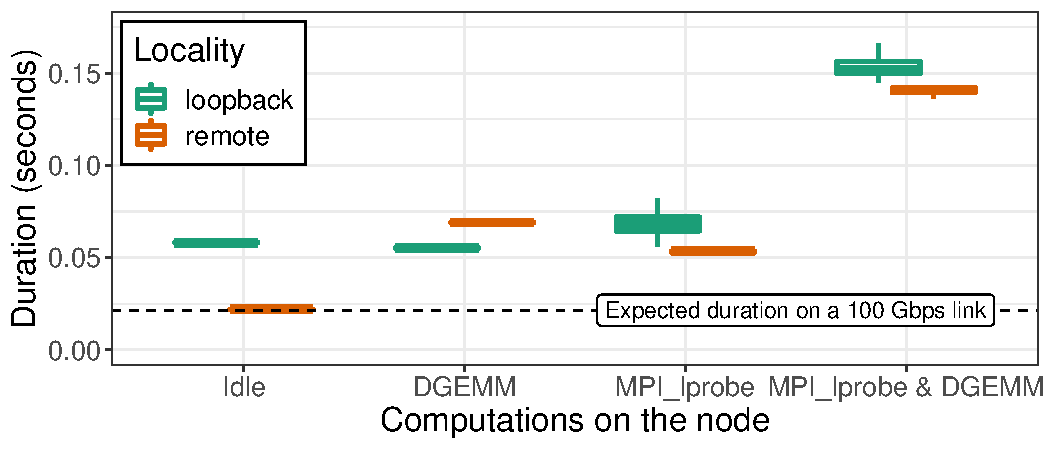
\includegraphics[width=1\linewidth]{img/experiment/experimental_conditions/communication_computation_interference.pdf}
            \caption{Durations of a call to \recv with a message of \NSI{256}{\mebi\byte} and different background
            activities.}%
            \label{fig:experiment:experimental_conditions}
        \end{figure}

        The background noise we introduced had a large effect on the performance of the ping-pong. The durations of
        individual calls to \recv are presented in Figure~\ref{fig:experiment:experimental_conditions}. Making simple
        calls to \dgemm in the background increases the remote duration by nearly a factor \(3\), without affecting the
        local durations. The ring communication pattern with \texttt{MPI\_Iprobe} busy waiting increases both the local
        and remote durations, although the effect remains small for the local communication. Finally, adding \dgemm
        calls to the busy waiting increases a lot the durations of all communications, by adding an overhead of about
        \NSI{0.1}{\second}.

        Although we do not have a definitive explanation of the root cause of this phenomenon, it is extremely important
        to reproduce it in the calibration benchmark if we wish to have a faithful model.

	\section{Conclusion}
		%% TODO
        %% - Certains facteurs extérieurs peuvent grandement impacter l'expérience, exemple
        %%   des problèmes de température sur dahu-{13,14,15,16}. D'où la nécessité de (1)
        %%   contrôler d'avantage l'environnement et (2) collecter d'avantage
        %%   d'informations sur l'environnement.
        %% - La randomisation est très importante pour se prémunir de biais expérimentaux. Or, des fois on cherche
        %%   justement ces biais.
        %% - De manière plus générale, les conditions expérimentales ont un rôle très important.
        A common theme to several sections of this chapter was the importance of the randomisation. It is of great help
        to avoid or at least limit any experimental bias. We have presented several counter-intuitive phenomenons that
        were only revealed through the randomisation (or the lack thereof). However, in some cases, we needed our
        experiments to be biased, to have more realistic experimental conditions. When we execute a micro-benchmark that
        supposedly mimic a real application, the main objective is for this micro-benchmark to be the best possible
        surrogate for the real application, begin unbiased is only a secondary goal.

        During our work, we have been confronted multiple times to external factors that unknowingly affected our
        experiments (\eg cooling issues, BIOS upgrades). With this kind of artifacts, it can become more difficult to
        trust any experimental results, especially in the presence of unexpected phenomenons like the ones presented
        here. This demonstrates the great importance of gaining back this trust by (1) having an experiment engine to
        automatize everything (thereby limiting greatly the human errors) and collect relevant information and (2)
        making regular tests on the platform to detect eventual changes.

\chapter{Performance non-regression tests}%
\label{chapter:experiment:tests}
    %% TODO
    %% La partie précédente a montré que de nombreux problèmes peuvent survenir sur un
    %% testbed comme Grid'5000. Certains sont très visibles et vont être détectés
    %% rapidement (e.g. un disque HS), d'autres sont plus subtiles et peuvent passer
    %% inaperçu, faussant donc les expériences (e.g. performance inférieure de quelques
    %% pourcents). Dans cette partie, on essaye de détecter ces problèmes
    %% automatiquement.
    When working on the simulations described in Part~\ref{part:prediction}, we occasionally encountered inconsistent
    performance. The reasons are multiple, ranging from the hardware to the software. This motivated the implementation
    of performance non-regression tests, to help us detect any noteworthy change on the platform. In this chapter, we
    start by giving an overview of the existing state of the art and explaining the statistics we based our work on in
    Section~\ref{sec:state_of_art}. Then, in Section~\ref{sec:test:implementation} we describe how we implemented the
    tests, from the experiment execution to the final test result. We show and explain the graphical representation of
    our test results, and we describe the various events we were able to detect on Grid'5000 platform. Finally, in
    Section~\ref{sec:test:conclusion} we propose several ways to improve this work.
    \todo{We should discuss the normality assumption somewhere, I am not sure of the best location though.}

    \section{State of the art}%
    \label{sec:test:state_of_art}

        Testing is a core activity of software development. It is usually taught as soon as the first programming courses,
        students need to verify that their programs work as expected. More experienced software developers generally
        use a wide variety of techniques and methodologies to limit the presence of bugs.

        Performance testing is less common, the main reason being that it is arguably much more difficult than testing
        for correction.
        \begin{itemize}
            \item For a performance value to be meaningful, a lot of care needs to be taken when running the test for
                controlling the experimental environment.
            \item The result of a benchmark is a raw performance value (\eg a duration, an amount of memory or an amount
                of energy). Ultimately, the test should return a boolean, stating whether the test was successful or
                failed. It is difficult to define properly such a \emph{truth}. One could define an interval for the
                expected value, but this will most of the time be an arbitrary choice. A complementary solution, to
                ensure that the performance values remain stable throughout the life cycle of the software, would be to
                use statistical tests.
        \end{itemize}

        \subsection{Lack of tests}%
        \label{sub:lack_of_tests}

            %% TODO: check how to properly cite software. In particular, what contributors should we list?
            This section lists several examples of well established software projects with limited or even nonexistent
            performance testing.

            Simgrid~\cite{simgrid}, the simulation framework used in Part~\ref{part:prediction}, is a well established
            software. In the last twenty years, several dozens of contributors have helped to improve or extend it.
            Simgrid has also supported the research for several hundreds of articles, demonstrating a wide user base
            (relatively to its niche area). The main developers of Simgrid have spent countless hours in optimizing the
            speed of its core components, like the linear maxmin solver. Despite these efforts, there are currently no
            performance test in place to prevent eventual performance regressions.

            To the best of our knowledge, even HPC libraries like OpenBLAS~\cite{openblas} and OpenMPI~\cite{openmpi} do
            not use automated performance tests. OpenBLAS has several benchmarks
            implemented\footnote{https://github.com/xianyi/OpenBLAS/tree/f917c26e/benchmark}, but they rely on human
            intervention to run the tests and interpret the performance results. OpenMPI has a software, named
            MTT\footnote{https://open-mpi.github.io/mtt/}, to automatically deploy a middleware on an infrastructure and
            run correction tests as well as benchmarks. Yet again, the result of these benchmarks has to be interpreted
            by a human.

            SimdJSON~\cite{simdjson} is a state of the art C++ library to parse JSON documents extremely efficiently. It
            can process documents at about \NSI{2.5}{\giga\byte/\second}, more than twice faster than the concurrent
            JSON parsers. It is widely used, with more than twelve thousand stars on Github. Yet, in April 2020, one of
            the main contributors submitted an issue\footnote{\url{https://github.com/simdjson/simdjson/issues/812}} to
            report a previously unnoticed \NSI{50}{\percent} performance drop when the library was compiled with Visual
            Studio 2019 instead of G++ 7.5.0. This shows that even high performance libraries do not always have the
            methodology and tools to avoid performance regressions.

        \subsection{Existing work}%
        \label{sub:existing_work}

            \subsubsection{Benchmarking software: testing code snippets}%

                Several libraries already exist for benchmarking C++ software. Catch2~\cite{catch2} is a widely used
                unit testing framework for C++. It also provides basic functionalities for benchmarking code snippets.
                Several alternatives exist, developed specifically for C++ benchmarking~\cite{celero,hayai,nonius}, but
                seemingly no longer maintained and with a smaller user base.

                Google Benchmark~\cite{google-benchmark} is a C++ library to benchmark code snippets. It is well
                established with several dozens of contributors and about \Num{5000} stars on Github. It greatly
                facilitates the creation of parametric micro-benchmarks by adding only a few lines to an existing code.
                The result can be pretty-printed in the terminal or written in a file in a CSV or JSON format. It is
                even possible to automatically compute the asymptotic complexity. Finally, they provide a
                script\footnote{https://github.com/google/benchmark/blob/8f5e6ae0/tools/compare.py} to compare the
                results of two executions of the same benchmark, it will print the difference with a raw value as well
                as a percentage.  If there is a large enough number of repetitions of these benchmarks, the script can
                also perform a Mann–Whitney U test to test if the performance for these two series of runs is
                statistically identical.

                All these libraries suffer from at least one of the following limitations:
                \begin{itemize}
                    \item For a given code snippet and a given input, they will perform several iterations and report
                        the average duration. The user has no control on this number of iterations which is not even
                        deterministic, as the code snippet is executed in a loop for a fixed period of time.
                    \item We do not have any information on the distribution of these durations, only the average is
                        reported, the standard deviation is not displayed and we do not have any confidence interval for
                        the estimations of the mean. Note that this is understandable, these libraries typically start a
                        timer, then perform the iterations, they never measure the duration of an individual iteration.
                        It makes sense when measuring an extremely short code snippet that can take a few nanoseconds,
                        but this is more unfortunate in our use case where we measure longer function calls that take at
                        least several milliseconds.
                    \item There is no support for randomization, the code snippets are executed in a deterministic
                        order.  The calls to a given snippet with different parameters are also executed in a
                        deterministic order.
                    \item The statistical tests implemented (if any) are quite basic.  There is also no graphical
                        visualization of the results, which would greatly help the user to (1) better understand the
                        outcome of the test (not everyone knows what is a \emph{P-value}) and (2) visually detect
                        eventual differences not captured by the test (the Anscombe's quartet is the classical example).
                    \item There is no support for comparing long-term performance evolution. With these libraries, it
                        is possible to make performance measures for a given state of the codebase on a given machine.
                        It is even possible to make point-to-point comparison with Google Benchmark, \ie to compare two
                        states of the codebase or two machines. However, we still miss the full picture, the variation
                        of the performance on an historical timeframe.
                \end{itemize}

            \subsubsection{Benchmarking software: long-term performance evolution of an application}%

                Another interesting work is related to the StarPU project~\cite{AugThiNamWac11CCPE}. StarPU is a state
                of the art C/C++ task programming library that handles task dependencies and optimized usage of
                resources (heterogeneous scheduling and data transfers). It is also possible to accurately simulate a
                StarPU application, using the Simgrid simulation framework~\cite{stanisic:hal-01147997}. As part of
                their development methodology, the StarPU team performs nightly runs of a few selected StarPU
                applications and measure their performance, both in reality and in simulation. The goal is to detect any
                performance regression eventually introduced by a change in the software.
                Figure~\ref{fig:non_regression:state_of_art:starpu} presents the temporal evolution of the StarPU
                implementation of \texttt{spotrf}, which computes a Cholesky factorization of a given matrix. The green
                line is the observed performance in reality, the orange line is the estimation made in simulation. The
                large jump on 15/12/2017 is due to a hardware upgrade. The real runs exhibit an extremely large
                variability, which are mainly experiment artifacts: some experiments were performed on a badly
                configured node which does not report the correct number of cores, so StarPU cannot use appropriately
                the machine.  Since the StarPU team is interested in detecting regressions in StarPU itself and not the
                platform, these simulations are extremely valuable to them, they allow to rule out the false conclusions
                that would be made by looking only at the real runs.
                \begin{figure}[htpb]
                    \centering
                    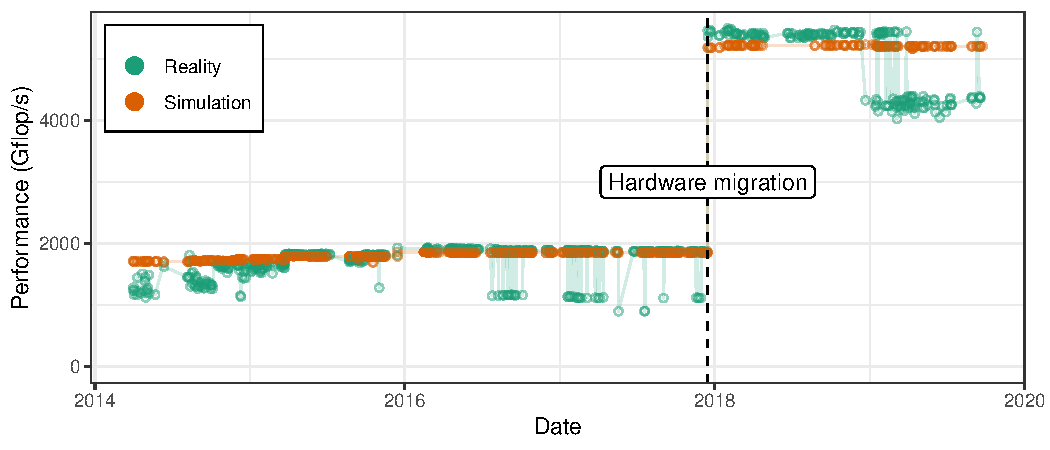
\includegraphics[width=\linewidth]{img/experiment/non_regression/state_of_art/starpu_new.pdf}
                    \caption{Evolution of the performance of a StarPU implementation of \texttt{spotrf} function, both
                    in reality and in simulation~\cite{thibault:hal-02943753}.}%
                    \label{fig:non_regression:state_of_art:starpu}
                \end{figure}

                The approach of the StarPU team is particularly interesting, because they executed their application on
                a controlled environment on a near-daily basis for several years. An important issue however is that they
                did not perform any statistics, they only relied on a visual inspection of the plot to decide whether
                the last modifications of their codebases had any significant effect on performance. While this can be
                satisfying to some extent, this raises two concerns:
                \begin{itemize}
                    \item They could miss a subtle change in the performance or detect it much later, as it can be
                        extremely difficult and error-prone. \footnote{Emery Berger uses the term "eyeball statistics":
                        \url{https://youtu.be/r-TLSBdHe1A}}
                    \item This does not scale well, adding more applications or running the test on more machines would
                        make this inspection very tedious.
                \end{itemize}

            \subsubsection{Benchmarking systems}%

                Other tools exist for measuring the performance of a platform under some workload. Here, we are not
                interested in the execution of a given software, but rather the whole platform, \ie the combination of
                the hardware, the operating system and eventual programs running concurrently on the system.
                High Performance Linpack \cite{hpl} is such a tool, it performs a dense linear algebra operation using
                one or several computers and reports the observed flop rate.

                Another system benchmarking tool is stress-ng\cite{stress-ng}. It runs a selected workload for a given
                duration and reports various aggregated performance. Over 240 different stress tests are implemented and
                can be combined (\eg it is possible to launch three processes that perform a lot of I/O operations and
                five processes that are CPU-intensive with vectorized floating point operations). The reported metrics
                include the duration, but also the number of instructions, the number of cache reads and writes, the
                number of page faults, etc. Several dozens of bugs have been found in the Linux kernel thanks to the use
                of this benchmark.

                These libraries suffer from the same limitations previously described: there is no randomization when
                several configurations are combined, and no statistical tests are available.

                The Grid'5000 platform already has tests in place. First, a script called \texttt{g5k-checks} verifies
                each time a node boots that its characteristics match the reference information (\eg the amount of
                memory, the BIOS version). Additionally, more extensive tests are executed on a regular basis on all the
                nodes \cite{nussbaum:hal-01538682}. These are mostly \emph{correction} tests, they perform several
                operations (\eg node deployment, network reconfiguration) that can either succeed or fail. Two
                \emph{performance} tests are implemented, one for the network bandwidth, the other for the disk
                bandwidth.  However, they use threshold values to define what is an acceptable performance, hence they
                will detect a severe regression but will miss more subtle changes.

        \subsection{Statistical test}%
        \label{sub:statistical_test}

            In this section, we describe how to compute a prediction region for multivariate normal variables. This will
            then be used to implement a statistical test.  This section is mostly based on Section 4.4 of
            Chew~\cite{chew}.\footnote{This publication, dating from 1966, is the oldest paper used in this thesis. It
            has been written by an employee of RCA Service Co., a contractor of the US Air Force. The author of the
            paper describes the typical use case: computing the coordinates of a prediction ellipse for the splash point
            of a future missile shot. I believe this is a poor usage of statistics.}
            \begin{quote}
                Suppose that we have already observed \(n\) vectors of dimension \(p\): \(\bm{x_1},\dots,\bm{x_n} \in
                \mathbb{R}^p\). We define the random variable \(\bm{m}^{(r)}\) to be the sample mean of the next (unknown)
                \(r\) observations: \(\bm{m}^{(r)}= \frac{\bm{x_{n+1}}+\dots+\bm{x_{n+r}}}{r}\). We assume here that all the
                \(\bm{x_i}\) are independent and identically distributed according to a multivariate normal distribution
                of unknown mean and covariance matrix.

                Then, the prediction region of \(\bm{m}^{(r)}\) with probability \(\gamma\) is:
                \begin{equation}\label{eqn:experiment:non_regression:pred_region}
                    \frac{nr}{n+r} (\bm{m}^{(r)} - \overline{\bm{x}})^T \bm{S}^{-1}(\bm{m}^{(r)} -
                    \overline{\bm{x}})
                    =
                    \frac{(n-1)p}{n-p} Q_F(1-\gamma, p, n-p)
                \end{equation}
                Where \(\overline{\bm{x}}\) and \(\bm{S}\) are respectively the sample mean and sample covariance matrix of
                the \(n\) observed \(\bm{x_i}\), and \(Q_F(\alpha,v_1,v_2)\) denotes the upper \(\alpha\) quantile of
                \(F(v_1, v_2)\), the F-distribution with \(v_1\) and \(v_2\) degrees of freedom.
            \end{quote}

            We therefore propose the following statistical test for \(\bm{m}^{(r)}\) with confidence \(\gamma\). First,
            compute the value:
            \begin{equation}\label{eqn:experiment:non_regression:test}
                t = \frac{nr(n-p)}{(n+r)(n-1)p} (\bm{m}^{(r)} - \overline{\bm{x}})^T \bm{S}^{-1}(\bm{m}^{(r)} -
                \overline{\bm{x}})
            \end{equation}

            Then, raise an error if \(t \geq Q_F(\gamma, p, n-p)\).  Note that there is no closed form for the value
            \(Q_F\), but it can be obtained (numerically) in R with the function
            \texttt{qf}\savefootnote{footnote:R_fdist}{\url{https://stat.ethz.ch/R-manual/R-devel/library/stats/html/Fdist.html}} and in Python
            with the function
            \texttt{scipy.stats.f.ppf}\savefootnote{footnote:PY_fdist}{\url{https://docs.scipy.org/doc/scipy/reference/generated/scipy.stats.f.html}}.

            The proposed test is illustrated in Figure~\ref{fig:non_regression:stat:single_point}. A large number of points,
            in black, have been generated according to a known bivariate normal distribution. Their abscissa (resp.
            ordinate) are distributed according to a normal distribution of mean \(\mu_x\) and standard deviation
            \(\sigma_x\) (resp. \(\mu_y\) and \(\sigma_y\)). The abscissa and ordinates of the points are not independent,
            they have a correlation coefficient of -0.7. The \NSI{99.5}{\percent} prediction regions are shown in blue. Two
            additional points are shown in the scatter plot, representing new observations. The orange point has coordinates
            \((\mu_x+2\sigma_x,\mu_y+2\sigma_y)\) and the green point has coordinates \((\mu_x+2\sigma_x,\mu_y-2\sigma_y)\).

            If each dimensions were considered independently, we would conclude that the probabilities to observe the orange
            point or the green point are equal. Indeed, these two points have equivalent positions in the one-dimension
            density graphs and they both fall within the \NSI{99.5}{\percent} interval. Now, when we look at both dimensions
            simultaneously, the green point becomes much more likely to be observed, it is within the blue ellipse while the
            orange point is outside.

            \begin{figure}[htpb]
                \centering
                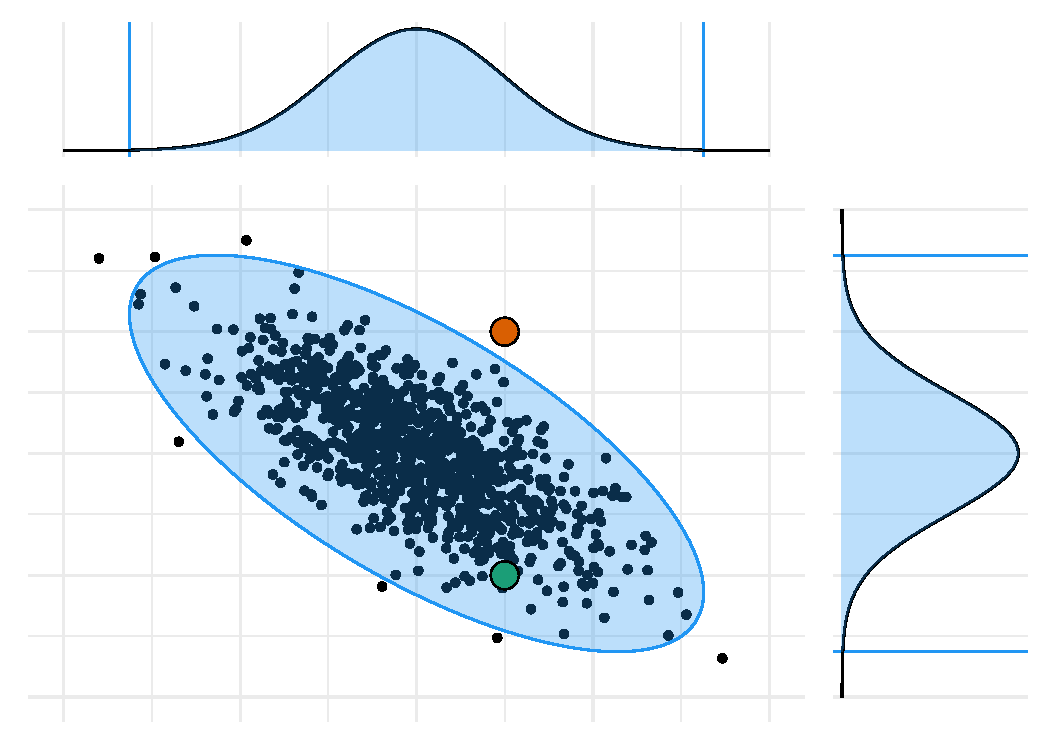
\includegraphics[width=0.9\linewidth]{img/experiment/non_regression/statistics/single_point.pdf}
                \caption{Illustrating the proposed test with two sets of one observation (\(r=1\)) and a bivariate normal
                distribution (\(p=2\)). The blue zones represent the \NSI{99.5}{\percent} prediction regions.}%
                \label{fig:non_regression:stat:single_point}
            \end{figure}

            In Figure~\ref{fig:non_regression:stat:several_points}, two sets of five additional observations are presented
            as colored dots. Individually, they were all likely to be observed, they are within the dashed ellipse
            representing the \NSI{99.5}{\percent} prediction region for a single point (\ie \(r=1\)). However, if we
            consider them together, the prediction region for their averages shrinks drastically. Now it becomes clear that
            the set of green points was more likely to be observed than the set of orange points, the green average (marked
            by a cross) is within the filled ellipse representing the \NSI{99.5}{\percent} region for a five-point average
            (\ie \(r=5\)) whereas the orange average is outside.

            \begin{figure}[htpb]
                \centering
                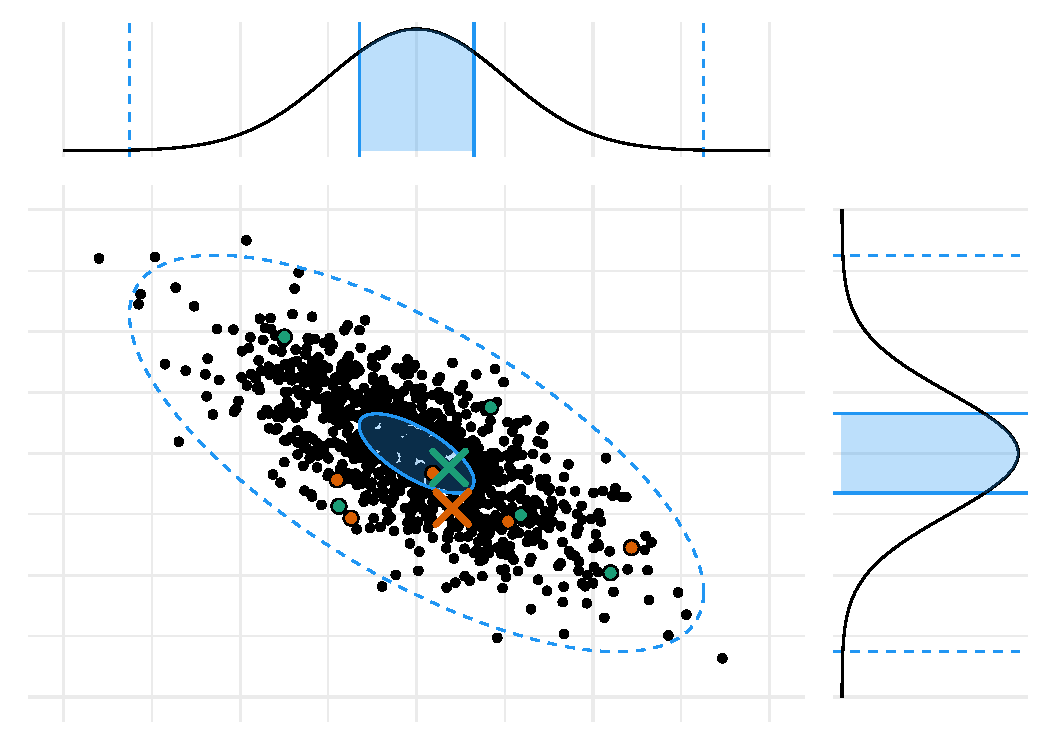
\includegraphics[width=0.9\linewidth]{img/experiment/non_regression/statistics/several_points.pdf}
                \caption{Illustrating the proposed test with two sets of five observations (\(r=5\)) and a bivariate normal
                distribution (\(p=2\)). The blue dashed lines represent the \NSI{99.5}{\percent} prediction regions for
                single observations, the blue zones represent the \NSI{99.5}{\percent} prediction regions for the averages of
                five new observations, represented by crosses.}%
                \label{fig:non_regression:stat:several_points}
            \end{figure}

            % TODO discuss the choice of the distribution. Normal vs F distribution. Should we even use this at all? Why
            % not simply the Z-score? See the entries from 2020-05-{07,11,13} in my journal.

    \section{Implementation of the test}%
    \label{sec:test:implementation}
        %% TODO
        %% Description du workflow mis en place, avec un joli dessin.
        %% - Génération du fichier d'expérience.
        %% - Soumission de jobs sur chaque cluster.
        %% - Réalisation de l'expérience, entièrement gérée par peanut.
        %% - Push automatique des résultats sur le dépôt gitlab.
        %% - Soumission d'un job CI pour extraire et agréger les informations des archives.
        %% - Réalisation des tests et courbes sur les données.
        %% - Aussi montrer la distribution des données des clusters (e.g. perf vs frequence) avec les ellipses.
        \subsection{Workflow}%
        \label{sub:workflow}

            This section describes the different steps and tools involved to perform this performance test, from the
            execution of the experiment on the target machines to the generation of the final plots. It discusses
            several technical choices that have been made and gives some insights to their advantages and limitations.

            The workflow consists in three main steps:
            \begin{description}
                \item[Experiment execution] The \dgemm calibration program is executed on the desired nodes. We obtain
                    a \texttt{zip} archive containing the experiment data and metadata.
                \item[Archive extraction and aggregation] The data is extracted from the archive and appended to two
                    \texttt{hdf5} files (one for the \dgemm duration, one for the monitoring data). Then, some
                    statistics are computed with this new data on a per-CPU and per-experiment basis (\eg average \dgemm
                    performance and average CPU temperature), these aggregated values are added to two \texttt{csv}
                    files.
                \item[Statistical test computation] Several statistical tests are done on the sequence of aggregated
                    data. The result is presented as several \texttt{jupyter} notebooks containing plots.
            \end{description}

            \subsubsection{Experiment execution}%

                The experiment script is written in Python and uses the Peanut experiment
                engine\footnote{\url{https://github.com/Ezibenroc/peanut}} (see
                Section~\ref{sec:peanut}). This is also the script used to perform the \dgemm calibrations for HPL
                simulation (see Part~\ref{part:prediction}).

                On a regular basis, typically three to four times a week, we use this script to submit new experiment
                jobs to Grid'5000's scheduler. This regular submission could have been easily automatized, \eg with
                \texttt{cron} or \texttt{systemd}, but we made the choice to keep this step manual. By inspecting the
                Grid'5000 Gantt chart, we can check whether the clusters are currently heavily used or not and decide if
                we should postpone or experiment to avoid disturbing too much the other users. A particularly good
                timeframe for our experiments is usually between 7 a.m. and 9 a.m., when the (longer) nightly
                experiments have terminated and the (shorter and interactive) daily experiments have not started yet.
                We generally submit one job per cluster, requesting all the nodes, but we sometimes have to split the
                experiments and make several smaller jobs when only a subset of the nodes is free immediately. The
                alternative would be to submit the full-scale job anyway, but it would get scheduled later in the day,
                which might disturb other users that need to work interactively on some nodes. Again, this kind of
                decisions is the reason why this step is not trivial to automatize.

                When scheduled, the experiment script will perform the following steps:
                \begin{enumerate}
                    \item Deploy a fresh Debian image on all the nodes of the job and install the required dependencies.
                    \item Apply the desired setup to the nodes (\eg enable turboboost, disable hyperthreading, use the
                        lowest C-state and P-state).
                    \item Start the node monitoring script in the background.
                    \item Perform a stress of \NSI{10}{\minute} on the nodes as a warm-up.
                    \item Run the \dgemm calls with the desired experiment file.
                    \item Collect the resulting data (two CSV files, one for \dgemm durations and one for monitoring
                        values) and meta-data (system files, software versions, etc.) and build an archive.
                    \item Push the archive to the git repository.
                \end{enumerate}

                The choice to use a git repository for storing the experiment data can seem peculiar, git is a very good
                version control system for small text files but is not the best choice to store gigabytes of data
                (although we mitigated this by using git LFS). It would have been undoubtedly more efficient to setup a
                proper database server for this task, but probably longer to implement.

                The \dgemm CSV file contains one row for each individual \dgemm call. The columns are the hostname of
                the node, the core ID, the exact time at which the call was made, the duration of the call and the
                \dgemm parameters (including the matrix sizes \(M\), \(N\) and \(K\)).

                The monitoring CSV file contains one row per sample, which typically happens every \NSI{5}{\second}. The
                columns are the hostname of the node, the exact time at which this sample was taken, then one column for
                each available metric (\eg temperature of the CPU n°1, frequency of the core n°6, power consumption of
                the CPU n°0).

            \subsubsection{Archive extraction and aggregation}%

                Once the experiments of the day have terminated, we submit an \emph{extraction} job on Grid'5000. In the
                first versions of this work, this step used to be implemented with Gitlab's continuous-integration, but
                this quickly revealed to be too demanding for the runner of our Gitlab instance.

                The extraction job is a small script that uses
                Cashew\footnote{\url{https://github.com/Ezibenroc/cashew}}, a Python library implemented specifically
                for this task. It performs the following steps:
                \begin{enumerate}
                    \item Clone the git repository.
                    \item Iterate on all the new archives to extract the performance and monitoring data. Append it to
                        the two \texttt{hdf5} data files.
                    \item Process the new additions in the data files to produce aggregated values, append these
                        aggregated values to the \texttt{csv} files.
                    \item Push the changes to the git repository.
                \end{enumerate}

                In the extraction step, we use the archive metadata to add some information to the tables stored in the
                two CSV files. For instance, we add the ID of the job and its scheduled date, the cluster of the node
                and a hash of the experiment file. We also reshape the monitoring table to switch from its wide format
                to a long format (\ie each row now has a set of identifier variables and a single measure variable).
                These two tables are then appended to the two \texttt{hdf5} files.

                We compared several alternative file formats to store this data: a simple CSV file, a CSV file
                compressed with \texttt{zip}, SQLite~\cite{sqlite}, Apache Arrow~\cite{arrow} and HDF5~\cite{hdf5} with
                various options. The Apache Arrow library had the fastest read and write operations as well as the
                smallest file. HDF5 with the \texttt{table} format and the \texttt{zlib} compression algorithm was the
                second best, the other alternatives were largely inferior in terms of I/O speed and disk footprint. Two
                important features of HDF5 made it preferable to Apache Arrow for our use case:
                (1) The possibility to append data to a file. With Appache Arrow, for each new experiment we would have
                to read the whole file in memory to add the new data.  (2) The ability to load only a subset of the data
                based on a logical predicate. For instance, it is possible to load the measures made on a given node
                between two given dates without having to read the whole file.

                In the aggregation step, we summarize the data from a given experiment into a single row for each CPU of
                each node. We keep the \dgemm data and the monitoring data separated. Both these files have identifier
                columns: cluster name, node ID, CPU ID, job ID, experiment start time and experiment file hash. Their
                measure columns are listed below:
                \begin{itemize}
                    \item In the \dgemm file, each row has the observed \texttt{dgemm} performance, computed as the
                        total number of flops (equal to \(2\sum_i M_iN_iK_i\)) divided by the total duration. Each row
                        also has the coefficients of the linear regression using the full polynomial model, as discussed
                        in Part~\ref{part:prediction}.
                    \item In the monitoring file, each row has the observed mean temperature, frequency, CPU power
                        consumption and DRAM power consumption. To represent the steady state of the experiment, these
                        averages are computed on a subset of the available values, a window starting \NSI{2}{\minute}
                        after the start of the \dgemm calibration program and ending \NSI{2}{\minute} later.
                \end{itemize}

            \subsubsection{Statistical test computation}%

                When the extraction and aggregation of the new data is terminated, we compute the statistical test. This
                is usually done in the same Grid'5000 job as the previous step, but it can be done independently, the
                test does not need the full repository, it automatically downloads the required files.

                The implementation directly follows the formula described in Section~\ref{sub:statistical_test}. It
                relies heavily on Numpy and Pandas for a better efficiency.

                Several factors are available. They are all tested independently, as a one-dimensional variable (\ie
                \(p=1\)). For each of them, two tests are realised, one with a window of one job (\ie \(r=1\)) and one
                with a window of five jobs (\ie \(r=5\)). The different factors are:
                \begin{description}
                    \item[Performance] Average \dgemm performance, including all calls. We recall that it is computed as
                        the total number of flops (equal to \(2\sum_i M_iN_iK_i\)) divided by the total duration. This
                        is not equal to the arithmetic mean of the individual performance values.
                    \item[Performance$_{\text{2048}}$] Average \dgemm performance, restricted to the calls with matrices
                        of size \(2048\times2048\).
                    \item[Frequency] Average CPU frequency during the \dgemm calls.
                    \item[Power$_{\text{CPU}}$] Average CPU power consumption during the \dgemm calls.
                    \item[Power$_{\text{DRAM}}$] Average DRAM power consumption during the \dgemm calls.
                    \item[Temperature] Average CPU temperature during the \dgemm calls.
                    \item[Model] All the parameters of the linear regression for the \dgemm durations, \ie the intercept
                        and the coefficients for the variables \(MNK\), \(MN\), \(MK\), \(NK\), \(M\), \(N\) and \(K\).
                        The regression parameters of the linear regression for \dgemm variability are also available.
                \end{description}

                A multi-dimensional test is also performed on the eight parameters of the linear regression for \dgemm
                durations (\ie \(p=8\)).
                An overview of the graphical presentation of these test results is presented in section
                \ref{sub:presentation_of_the_test_results}.

                As for the previous step, the test is implemented in Cashew and uses a Jupyter notebook. This notebook
                is instantiated and executed several times, once per cluster and per factor. All these copies are then
                converted to HTML and deployed to a website.

        \subsection{On the normality assumption}%
        \label{sub:on_the_normality_assumption}

            The statistical test described in Section~\ref{sub:statistical_test} assumes that the data follows a normal
            distribution. In this section, we argue that all the variables described previously satisfy this hypothesis.

            \begin{itemize}
                \item The factors Frequency, Temperature, Power$_{\text{CPU}}$ and Power$_{\text{DRAM}}$ are all an
                    arithmetic mean of several dozens of values. It comes directly by the central limit theorem that
                    these averages follow a normal distribution.
                \item The Model factors (\eg MNK) are coefficients of an ordinary least-square linear regression (OLS).
                    The input data are the averaged \dgemm durations, for each distinct tuple \(M,N,K\), we compute the
                    arithmetical mean of the durations observed on all the cores of a given CPU. Thus, by the central
                    limit theorem, the input data has a normally distributed noise. Now, if we note \(\bm{X}\) the
                    \(n\times8\) matrix of regressors (each of the \(n\) rows is an observation, the 8 columns are the
                    products \(MNK, MN, MK, NK, M, N\) and \(K\) that were used for this observation) and we note
                    \(\bm{y}\) the vector of observed durations, the estimator of regression coefficients
                    \(\hat{\bm{\beta}}\) can be obtained by computing \(\hat{\bm{\beta}} = \left( \bm{X}^{\mathsf T}
                    \bm{X} \right)^{-1} \bm{X}^{\mathsf T} \bm{y} \).  By doing this regression, we assume that \(\bm{y}
                    = \bm{X}\bm{\beta} + \bm{\varepsilon}\) where \(\bm{\beta}\) is the true (unknown) vector of coefficients
                    and \(\bm{\varepsilon}\) is the normally distributed noise. It follows that the estimator
                    \(\hat{\bm{\beta}}\) is also normally distributed.
                \item The factors Performance and Performance\(_{2048}\) are defined as a ratio of two values, the total
                    number of operations divided by the total duration. The number of operations is constant, only the
                    duration is a random variable. Since it is itself the sum of individual durations, it follows a
                    normal distribution, by the central limit theorem. If we note the ratio as
                    \(R=\frac{F}{T+\varepsilon}\) where \(F\) and \(T\) are constant and \(\varepsilon\) is a random
                    normal noise, we have \(R = \left(\frac{F}{T}\right) \left(\frac{1}{1+\varepsilon/T}\right)
                    \approx \frac{F}{T}\left(1-\frac{\varepsilon}{T}\right)\). The last approximation is obtained by the
                    Taylor expansion, it holds because \(T \gg \varepsilon\), \ie the variability of the total duration
                    is small compared to its average. Since \(F\) and \(T\) are constant and \(\varepsilon\) is normally
                    distributed, it follows that \(R\) is also normally distributed.
            \end{itemize}

        \subsection{Presentation of the test results}%
        \label{sub:presentation_of_the_test_results}

            \subsubsection{Evolution plot}%

                The historical evolution of the mean performance of two nodes is presented in
                Figure~\ref{fig:experiment:non_regression:evolution_dahu}. Each point represents the observed
                performance on a given experiment. The vertical dashed lines denote changes in the platform that had a
                significant effect on at least one of the observed factors. The grey lines (with a label on bottom) are
                protocol changes, we modified the experiment in a way that affected the results. The orange lines (with
                a label on top) are events that happened on the platform regardless of our will.  The grey ribbon is the
                \emph{fluctuation interval}, we expect all the observations to fall within this interval with a given
                confidence (\NSI{99.99}{\percent} in this figure). The \emph{reference set} of observations used to
                compute this interval consists of past observations that were made after the last change. In other
                words, (1) we do not consider the observations that were made in the future and (2) each time we
                recognise a change and add a vertical line, the fluctuation interval gets reseted.

                The fluctuation interval for a new value \(\bm{m}^{(r)}\) (which is the sample mean of \(r\) new
                observations \(x_{n+1},\dots,x_{n+r}\), note that \(r=1\) in
                Figure~\ref{fig:experiment:non_regression:evolution_dahu}) follows a rewriting of
                Equation~\ref{eqn:experiment:non_regression:test} with a single dimension (\(p=1\)). Noting
                \(\overline{\bm{x}}\) (resp. \(\bm{s}^2\)) the sample mean (resp. sample variance) of the reference set,
                the fluctuation interval is defined as:

                \begin{equation}\label{eqn:experiment:non_regression:interval}
                    I = \overline{\bm{x}} \pm s \left(\sqrt{\frac{n+r}{nr}Q_F(\gamma, 1, n-1)}\right)
                \end{equation}

                Whenever an observation falls outside the fluctuation interval, it is detected as an anomaly. It is
                classified as either a positive anomaly and colored in red if it is larger than the sample mean, or it
                is classified as a negative anomaly and colored in blue if it is lower than the sample mean.

                It occasionally happens that a single observation is way outside the fluctuation interval (\eg on
                Figure~\ref{fig:experiment:non_regression:evolution_dahu26}, one experiment had a performance of
                approximately \NSI{23}{\giga\flop/\second} near the end of 2020). When this happens, we manually label
                this point as an outlier and remove it from the reference set: it will not be taken into account for
                computing the reference interval afterwards.

                \begin{figure}[htpb]
                    \centering
                    \subfigure[Performance evolution of node \emph{dahu-14}\label{fig:experiment:non_regression:evolution_dahu14}]{
                        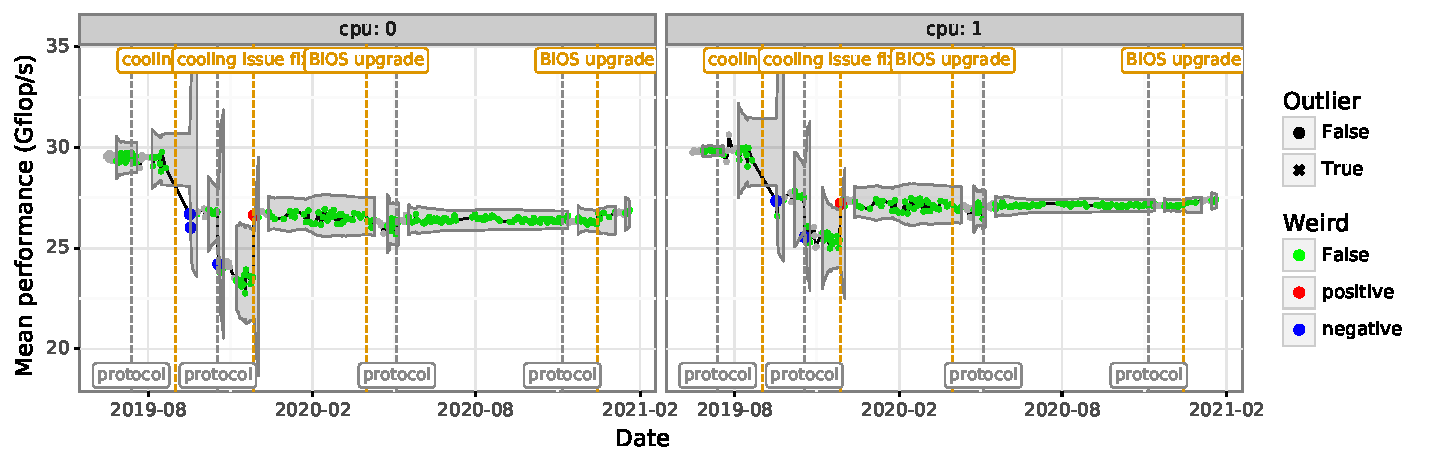
\includegraphics[width=\linewidth]{img/experiment/non_regression/implementation/evolution_dahu-14.pdf}
                    }
                    \subfigure[Performance evolution of node \emph{dahu-26}\label{fig:experiment:non_regression:evolution_dahu26}]{
                        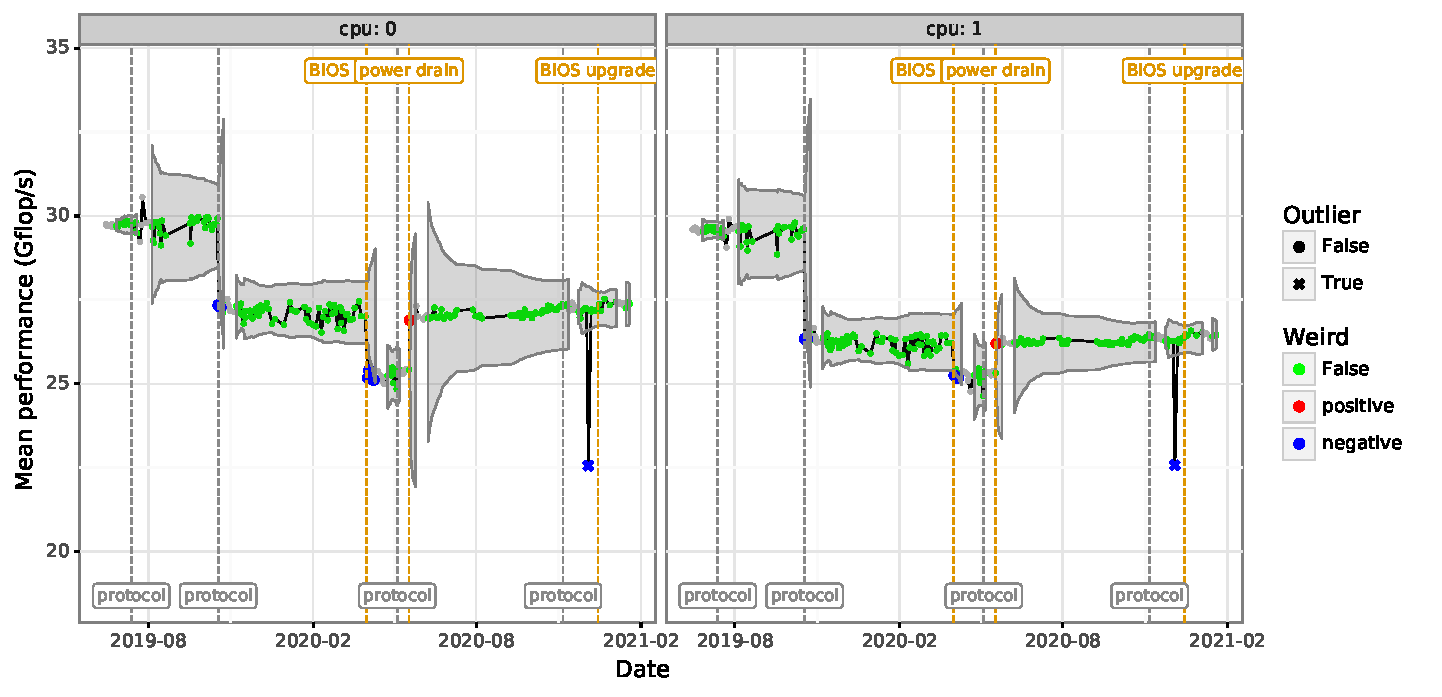
\includegraphics[width=\linewidth]{img/experiment/non_regression/implementation/evolution_dahu-26.pdf}
                    }
                    \caption{Evolution of the mean performance of the two processors of two nodes from cluster \emph{dahu}
                    (the fluctuation interval has a confidence of \NSI{99.99}{\percent})}%
                    \label{fig:experiment:non_regression:evolution_dahu}
                \end{figure}

            \subsubsection{Overview plot}%

                We are running regular tests for several factors on hundreds of nodes, it would be very long and tedious
                to review each individual plot. For this reason, we implemented overview plots, as presented in
                Figure~\ref{fig:experiment:non_regression:overview}. In this presentation, each processor of each node
                occupies one row. Individual experiments are still presented as points and the vertical grey or orange
                lines represent the same platform changes. We added intermediate levels in the colors to display how
                unlikely it was to make a given observation. In the one-dimension case (\ie \(p=1\)), this represents
                the distance between the observation and the sample mean of the reference set.

                More formally, this likelihood is the probability to make an observation at least as extreme. To compute
                it, we use the value \(t\) defined in Equation~\ref{eqn:experiment:non_regression:test} and define the
                likelihood \(\mathcal{L}\) as follows:
                \begin{equation}\label{eqn:experiment:non_regression:likelihood}
                    \mathcal{L} = 1-F_{F(p, n-p)}(t)
                \end{equation}
                Here, \(F_{F(v_1, v_2)}\) denotes the cumulative distribution function of the F-distribution with
                \(v_1\) and \(v_2\) degrees of freedom. An implementation is available in R with the function
                \texttt{pf}\repeatfootnote{footnote:R_fdist} and in Python with the function
                \texttt{scipy.stats.f.cdf}\repeatfootnote{footnote:PY_fdist}.

                \begin{figure}[htpb]
                    \centering
                    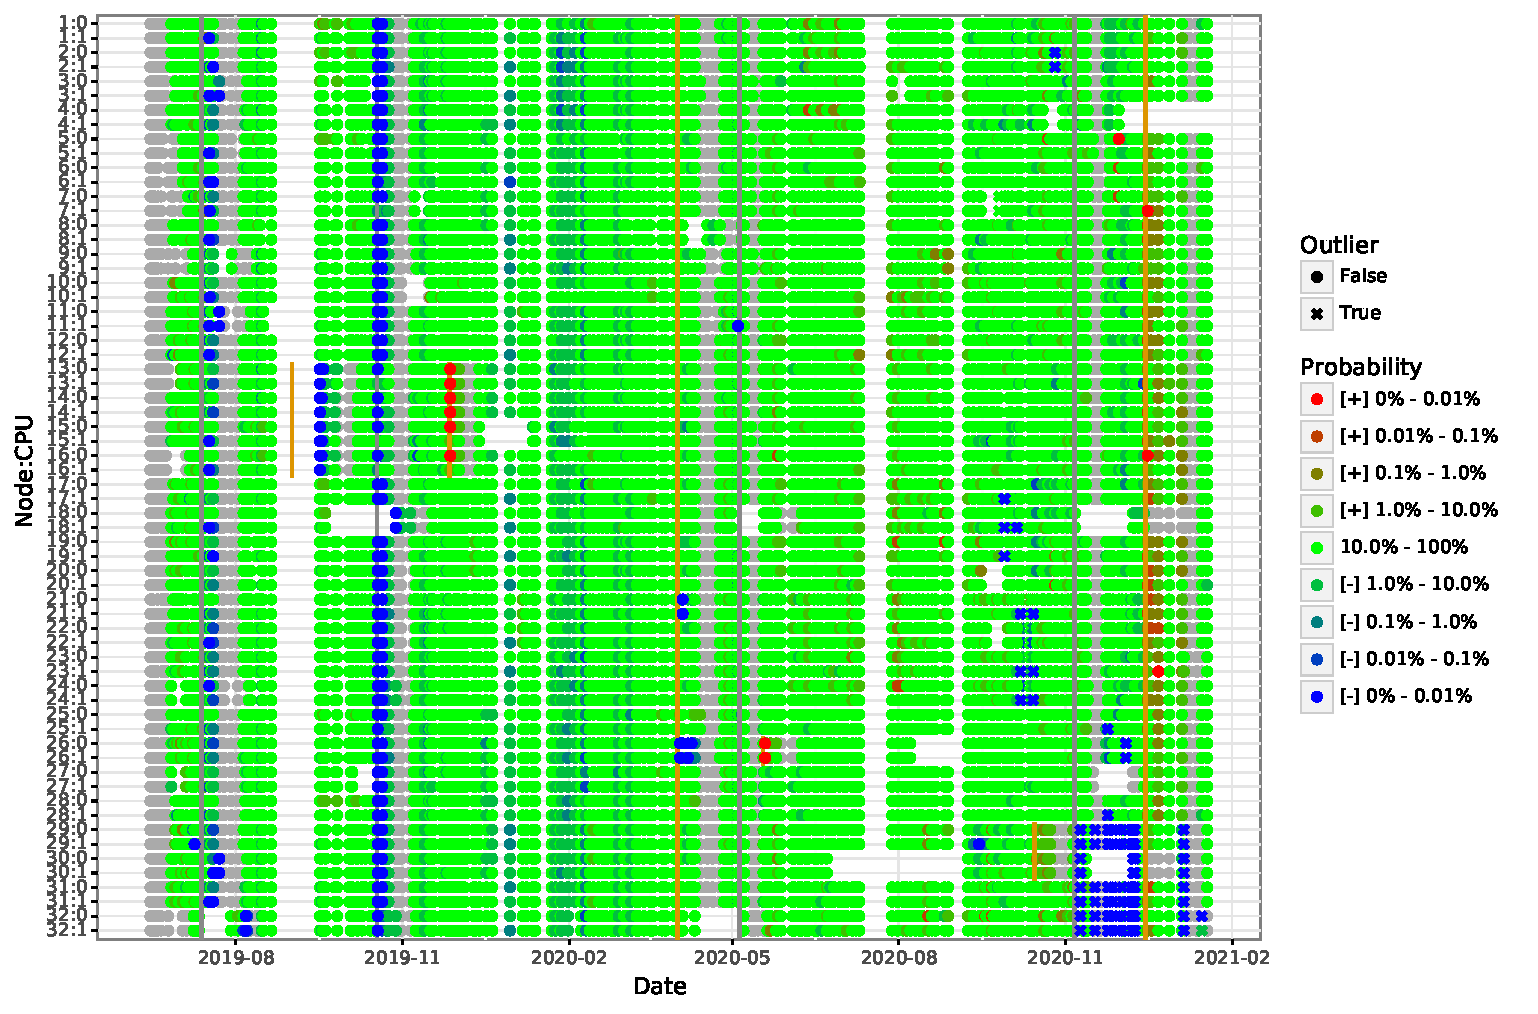
\includegraphics[width=\linewidth]{img/experiment/non_regression/implementation/overview.pdf}
                    \caption{Overview of the test result for the mean performance on cluster \emph{dahu}.}%
                    \label{fig:experiment:non_regression:overview}
                \end{figure}

            \subsubsection{Windowed test}%

                The test presented in Figure~\ref{fig:experiment:non_regression:overview} and
                Figure~\ref{fig:experiment:non_regression:evolution_dahu} was done with a single factor (\(p=1\)), for
                comparing a single new observation to the reference set (\(r=1\)). A similar test is implemented to
                compare five new observations to the reference set, still with a single factor (\(p=1\) and \(r=5\)).

                Figure~\ref{fig:experiment:non_regression:evolution_dahu_windowed} shows the performance evolution of
                two nodes of the cluster \emph{dahu} with the five experiment window. Taking the average of several runs
                reduces the noise. This allows to reduce considerably the width of the fluctuation interval, thereby
                permitting to detect much more subtle changes. The downside is that it introduces a lag, the change
                might not be detected immediately.

                \begin{figure}[htpb]
                    \centering
                    \subfigure[Performance evolution of node
                        \emph{dahu-14}\label{fig:experiment:non_regression:evolution_dahu14_windowed}]{
                        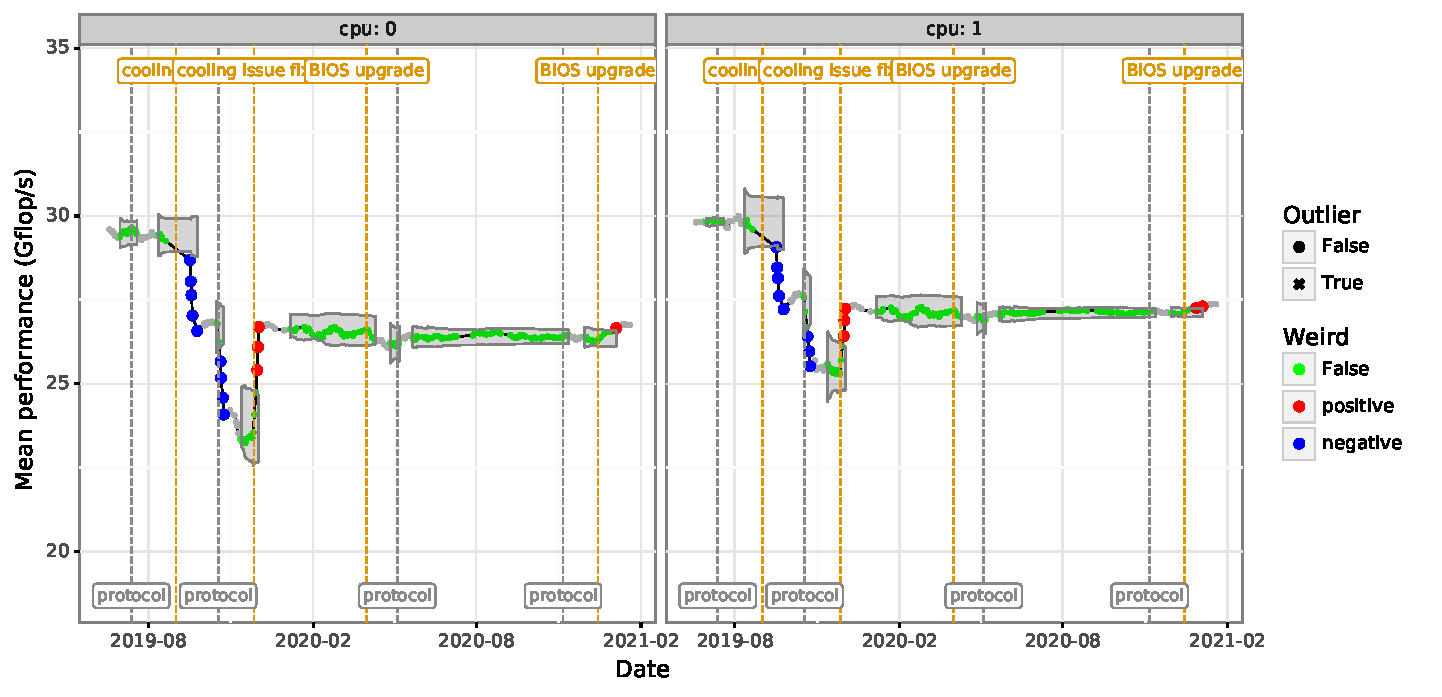
\includegraphics[width=\linewidth]{img/experiment/non_regression/implementation/evolution_dahu-14_windowed.pdf}
                    }
                    \subfigure[Performance evolution of node
                    \emph{dahu-26}\label{fig:experiment:non_regression:evolution_dahu26_windowed}]{
                        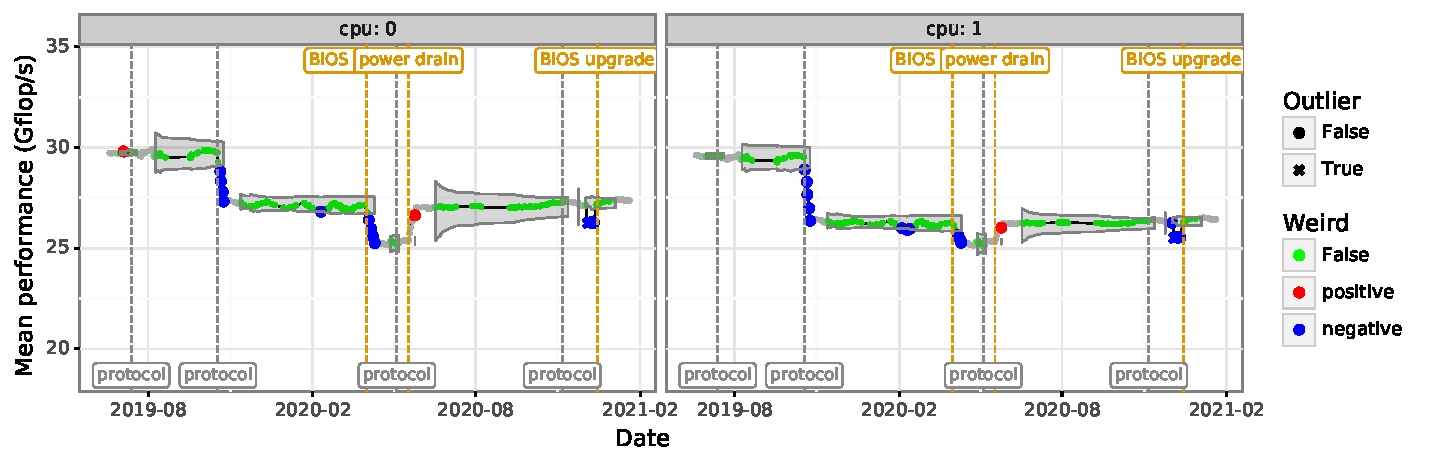
\includegraphics[width=\linewidth]{img/experiment/non_regression/implementation/evolution_dahu-26_windowed.pdf}
                    }
                    \caption{Evolution of the mean performance of the two processors of two nodes from cluster
                    \emph{dahu} using a window of five experiments (the fluctuation interval has a confidence of
                    \NSI{99.99}{\percent})}%
                    \label{fig:experiment:non_regression:evolution_dahu_windowed}
                \end{figure}

                The overview plot with the five experiment window is displayed in
                Figure~\ref{fig:experiment:non_regression:overview_windowed}. The vertical orange line on 2020/12/15
                marks a platform change we noticed. On this plot, it is very clear that the change has affected
                significantly a large fraction of the nodes by increasing their performance (positive anomaly). This was
                slightly visible on the non-windowed plot from Figure~\ref{fig:experiment:non_regression:overview}, but
                much more tenuous. This demonstrates well the complementarity of both tests: the non-windowed test is
                better for detecting quickly any large change, whereas the windowed test is best at detecting more
                subtle changes but with some lag.

                \begin{figure}[htpb]
                    \centering
                    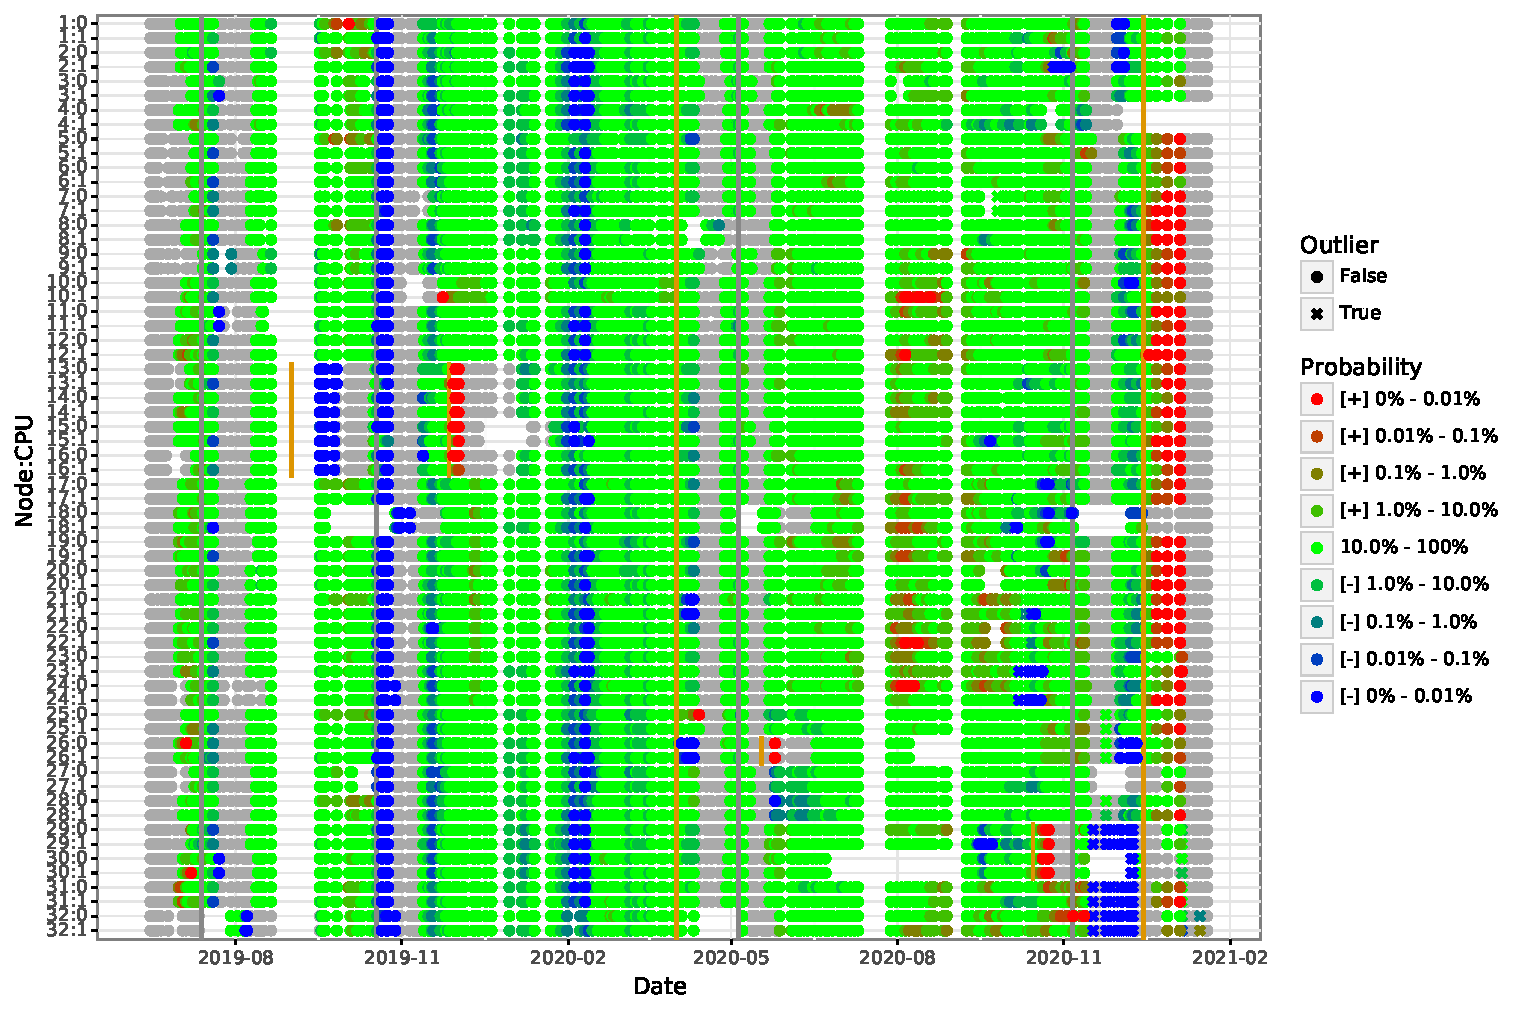
\includegraphics[width=\linewidth]{img/experiment/non_regression/implementation/overview_windowed.pdf}
                    \caption{Overview of the test result for the mean performance on cluster \emph{dahu} using a window
                    of five experiments}%
                    \label{fig:experiment:non_regression:overview_windowed}
                \end{figure}

            \subsubsection{Multi-factor test}%

                We have also implemented the multidimensional test.
                Figure~\ref{fig:experiment:non_regression:overview_multifactor} presents the overview plot for this test
                made on the eight regression parameters (\ie \(p=8\), the parameters are\(MNK, MN, MK, NK, M, N, K\) and
                the intercept). With several dimensions, there is no notion of \emph{negative} or \emph{positive}
                anomaly, hence all the detected anomalies are colored in red. Likewise, we cannot represent graphically
                the temporal evolution of these eight factors like we did in the single-dimension case.

                This figure should be compared to Figure~\ref{fig:experiment:non_regression:overview}, since both of
                them aim at detecting changes in \dgemm durations. We can notice two interesting differences:
                \begin{itemize}
                    \item The first change, which happened on 2019/07/13, was detected as very significant on all the
                        nodes with the multi-factor test. On the other hand, the single-factor test only marked a subset
                        of the nodes.
                    \item Two events have gone completely unnoticed by the multi-factor test whereas they were reported
                        by the single-factor test: the positive anomaly on \emph{dahu-26} from 2020/05/18, and the series of
                        negative anomalies (that we later decided to be outliers) between 2020/11 and 2020/12 on nodes
                        \emph{dahu-29}, \emph{dahu-30}, \emph{dahu-31} and \emph{dahu-32}. The reason they went
                        unnoticed is that a change was registered shortly before, so the reference set had a very low
                        number of points. The radius of our fluctuation region is proportional to \(Q_F(\gamma, p,
                        n-p)\), it is obviously not defined when \(n \leq p\). When \(n\) is larger than \(p\), the value
                        \(Q_F(\gamma, p, n-p)\) starts extremely high, then quickly decreases. Hence, although it is
                        defined, the test is not useful yet, we need to have a few more observations as reference.
                        The same problem obviously exists when \(p=1\), but we have to wait longer with a larger number
                        of parameters.

                        One way to limit this issue is to limit the number of factors used in the test. It appears that
                        only three of the regression parameters are really significant: \(MNK, MK\) and \(NK\). By doing
                        so, the multi-factor test is able to detect the anomaly from 2020/05/18 on \emph{dahu-26}, but
                        it still misses the outliers from 2020/11-2020-12.
                \end{itemize}
                \begin{figure}[htpb]
                    \centering
                    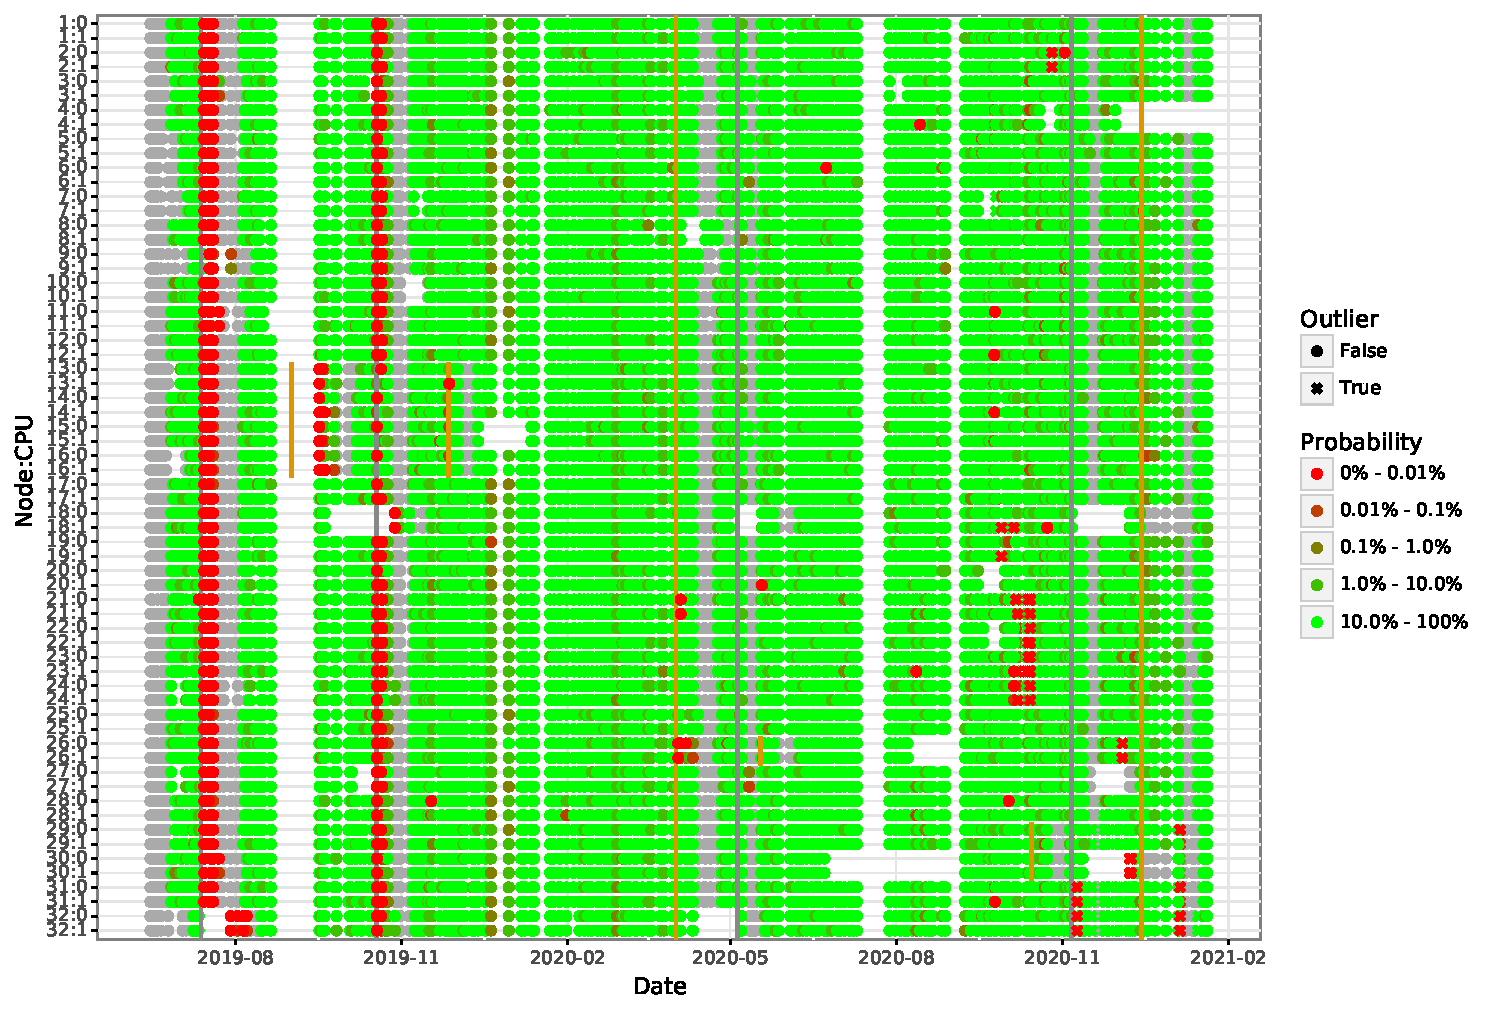
\includegraphics[width=\linewidth]{img/experiment/non_regression/implementation/overview_multifactor.pdf}
                    \caption{Overview of the test result for the eight regression parameters on cluster \emph{dahu}.}
                    \label{fig:experiment:non_regression:overview_multifactor}
                \end{figure}

            \subsubsection{Website presentation}%

                A screenshot of the landing page\footnote{The website presented here is publicly available at
                \url{https://cornebize.net/g5k_test/} and permanently archived at [...]\todo{Add a Zenodo link}} of the
                Grid'5000 performance tests we implemented is presented in
                Figure~\ref{fig:experiment:non_regression:home}. Each cluster is represented by a row, each factor by a
                column. Clicking on a button will open the test notebook for the desired cluster and factor. The last
                column is a drop-down menu showing all the coefficients for the linear regression, as well as a
                multi-dimensional test made on the first eight coefficients together.

                \begin{figure}[htpb]
                    \centering
                    \fbox{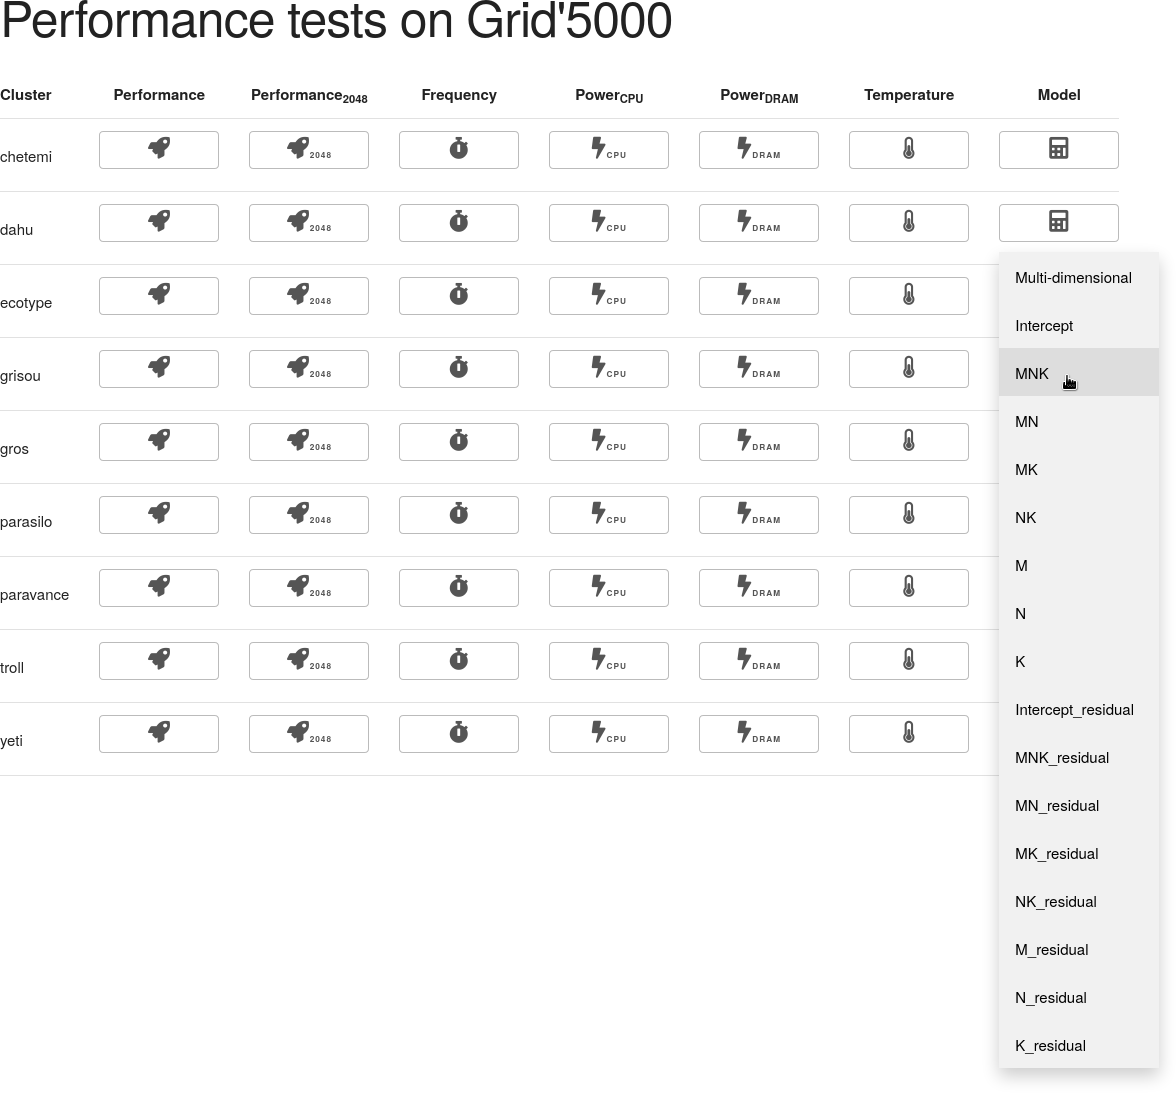
\includegraphics[width=\linewidth]{img/experiment/non_regression/implementation/g5k_test_home.png}}
                    \caption{Landing page of the test website.}%
                    \label{fig:experiment:non_regression:home}
                \end{figure}

                An extract of a single-factor notebook is presented in
                Figure~\ref{fig:experiment:non_regression:zoom_out}. The different parts of the notebooks are:
                \begin{enumerate}[label=\alph*]
                    \item This part is intended to import the required libraries and setup a few options, but most
                        importantly to define three variables: the desired cluster, factor(s) and confidence.
                    \item This is an histogram of the values obtained in the last run among the different processors of
                        the cluster for the desired factor. The average value as well as the spatial variability
                        coefficient are also displayed.
                    \item This is an overview plot of the cluster, similar to the overview plots previously presented.
                        The main difference is that the colors do not encode a test result, but the raw value. Like the
                        histogram, it helps to visualize the heterogeneity of the cluster. It also demonstrates once
                        again the utility of statistical tests: only the most brutal changes are visible in this plot,
                        the more subtle ones get completely unnoticed to the naked eye.
                    \item This is the non-windowed overview plot, as presented previously.
                    \item These are the non-windowed evolution plots, as presented previously.
                \end{enumerate}
                This notebook extract is obviously incomplete, only three evolution plots are shown. It also contains in
                a second part the windowed versions of the overview plot and evolution plots.

                % Note:
                % To make this figure, I took two screenshots of the g5k_test website on my desktop screen (2560x1440
                % resolution), using the "capture the current window" mode. Then, I cropped these screenshots with the
                % command:
                % convert input.png -crop 350x1310+30+103 output.png
                \tikzstyle{label}=[anchor=west]
                \begin{figure}[htpb]
                    \centering
                    \resizebox{!}{0.5\textheight}{\begin{tikzpicture}
                        \def\labelx{14}
                        \def\leftcolx{3}
                        \def\rightcolx{9}
                        \node[anchor=south west,inner sep=0] at (0,0)
                            {\hbox{\hspace{-.05\linewidth}\fbox{\resizebox{0.4\linewidth}{!}{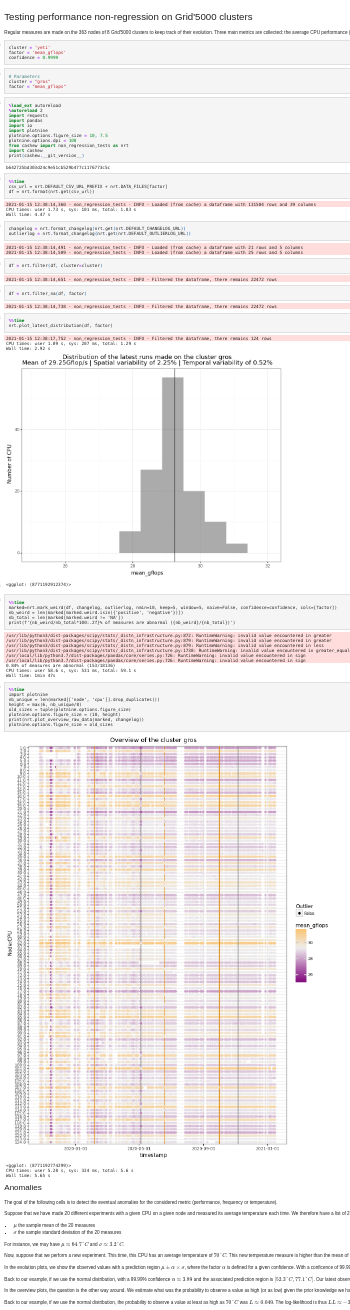
\includegraphics{img/experiment/non_regression/implementation/zoom_out1.png}}}\hspace{-.05\linewidth}}\vspace{-1em}};
                        \node[anchor=south west,inner sep=0] at (6,0)
                            {\hbox{\hspace{-.05\linewidth}\fbox{\resizebox{0.4\linewidth}{!}{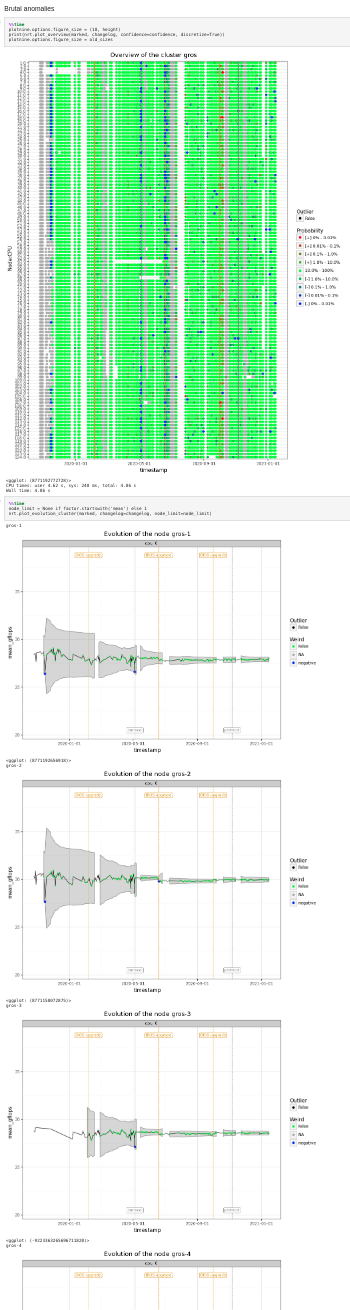
\includegraphics{img/experiment/non_regression/implementation/zoom_out2.png}}}\hspace{-.05\linewidth}}\vspace{-1em}};

                        \def\y{19.5}
                        \draw[-latex] (\labelx, \y) to (\leftcolx, \y) ;
                        \node[label, fill=white] at (\labelx, \y) {\textbf{(a)} Parameter definitions};

                        \def\y{18}
                        \draw[-latex] (\labelx, \y) to (\rightcolx, \y) ;
                        \node[label, fill=white] at (\labelx, \y) {\textbf{(d)} Cluster overview (test result)};

                        \def\y{14}
                        \draw[-latex] (\labelx, \y) to (\leftcolx, \y) ;
                        \node[label, fill=white] at (\labelx, \y) {\textbf{(b)} Cluster distribution in the last run};

                        \def\y{10}
                        \draw[-latex] (\labelx, \y) to (\rightcolx, \y) ;
                        \node[label, fill=white] at (\labelx, \y) {\textbf{(e)} Historical evolution of each node};

                        \def\y{5}
                        \draw[-latex] (\labelx, \y) to (\leftcolx, \y) ;
                        \node[label, fill=white] at (\labelx, \y) {\textbf{(c)} Cluster overview (raw value)};
                    \end{tikzpicture}}
                    \caption{Overview of a notebook (cluster \emph{gros}, average performance).}%
                    \label{fig:experiment:non_regression:zoom_out}
                \end{figure}

        \subsection{Detected events}%
        \label{sub:detected_events}

            Our non-regression tests have been used on a regular basis on nine Grid'5000 clusters during a period of
            several months (from July 2019 to February 2021 for \emph{dahu}, the first cluster we started to monitor).
            In total, we have tested 386 nodes (656 processors).

            The list and basic characteristics of these clusters is described in table
            \ref{tab:experiment:non_regression:clusters}. It has been curated from Grid'5000
            documentation\footnote{\url{https://www.grid5000.fr/w/Hardware}}.
            \begin{table}[htpb]
                \centering
                \caption{List of the Grid'5000 clusters covered by our tests.}
                \label{tab:experiment:non_regression:clusters}
                \begin{tabular}{l|llll}
                    Cluster & Nodes & CPU & Cores & Memory\\
                    \hline
                    chetemi   & 15  & \(2\times\) Intel Xeon E5-2630 v4  & \(2\times10\) & \NSI{256}{\gibi\byte}\\
                    dahu      & 32  & \(2\times\) Intel Xeon Gold 6130   & \(2\times16\) & \NSI{192}{\gibi\byte}\\
                    ecotype   & 48  & \(2\times\) Intel Xeon E5-2630L v4 & \(2\times10\) & \NSI{128}{\gibi\byte}\\
                    grisou    & 51  & \(2\times\) Intel Xeon E5-2630 v3  & \(2\times8\)  & \NSI{128}{\gibi\byte}\\
                    gros      & 124 & \(1\times\) Xeon Gold 5220         & \(1\times18\) & \NSI{96}{\gibi\byte}\\
                    parasilo  & 28  & \(2\times\) Intel Xeon E5-2630 v3  & \(2\times8\)  & \NSI{128}{\gibi\byte}\\
                    paravance & 72  & \(2\times\) Intel Xeon E5-2630 v3  & \(2\times8\)  & \NSI{128}{\gibi\byte}\\
                    troll     & 4   & \(2\times\) Intel Xeon Gold 5218   & \(2\times16\) & \NSI{384}{\gibi\byte}\\
                    yeti      & 4   & \(4\times\) Intel Xeon Gold 6130   & \(4\times16\) & \NSI{768}{\gibi\byte}\\
                \end{tabular}
            \end{table}

            We give in this section an exhaustive list of the events detected by running our tests.

            \subsubsection{BIOS upgrade}%

                The Grid'5000 technical team occasionally upgrades the BIOS and the firmware of all the nodes of a
                cluster. Most of the time, it does not affect the nodes in a noticeable way, but we did measure a
                significant change on several occasions.
                \begin{itemize}
                    \item On 2020/02/06, cluster \emph{gros}. The temperature of all the nodes increased by several
                        degrees. In a more subtle way, but still significant, the frequency and the \dgemm performance
                        have decreased on a large fraction of the nodes (T-test with a \NSI{95}{\percent} confidence).
                    \item On 2020/04/01, cluster \emph{dahu}. The upgrade caused a performance drop of \NSI{5}{\percent}
                        on node \emph{dahu-26}, as well as a decrease of its frequency and temperature. There was also a
                        statistically significant (albeit very small) change on the other nodes of the cluster (T-test
                        with a \NSI{95}{\percent} confidence). This issue on \emph{dahu-26} has later been resolved by
                        an administrator doing a power drain of the node. Note that this return to normal was also
                        detected by our tests.
                    \item On 2020/06/10, cluster \emph{gros}. All the nodes of the cluster had a performance drop of
                        about \NSI{1}{\percent}. The frequency has also dropped noticeably.
                    \item On 2020/09/29, cluster \emph{troll}. A very large temperature drop of temperature followed the
                        upgrade. The largest effect was on CPU n°1 of node \emph{troll-2}, where the temperature
                        decreased from \NSI{86}{\celsius} to \NSI{60}{\celsius}. Not all the processors of
                        the cluster encountered this temperature anomaly. In a more subtle but still significant way,
                        the \dgemm performance of several processors has increased. The frequency was not affected.
                    \item On 2020/10/01, cluster \emph{gros}. The average \dgemm performance of nearly all nodes had a
                        small but significant increase. The frequency has also slightly increased, whereas the
                        temperature was not affected.
                    \item On 2020/12/15, cluster \emph{dahu}. A large fraction of the nodes had a performance increase
                        of \NSI{1}{\percent}. The frequency also slightly increased and the temperature decreased.
                \end{itemize}

            \subsubsection{Cooling issue}%

                Four nodes from cluster \emph{dahu} encountered some issues in two occasions, namely \emph{dahu-13},
                \emph{dahu-14}, \emph{dahu-15} and \emph{dahu-16}. Their performance and frequency was lower by
                \NSI{10}{\percent} whereas their temperature was much higher, especially on their CPU n°0 where it went
                above \NSI{90}{\celsius} instead of the usual \NSI{20}{\celsius}. Our hypothesis is that for some
                unknown reason the cooling system of the nodes started to malfunction. It is interesting to note that
                the four nodes are located in the same chassis, which probably explain why they were all affected at the
                same time.

                This problem appeared a first time between October 2018 and March 2019. We did not perform regular
                measures on the platform at the moment, so we do not have a more precise timeframe. The issue was solved
                on 2019/05/15 by changing the node chassis.

                A few months later, the same issue happened again on the same four nodes, their performance and
                frequency had a very large drop and their temperature rose dramatically. We do not have an accurate date
                for this event, it could have happened between 2019/08/20 and 2019/09/16. The problem was solved on
                2019/11/27 as a side effect of some work done in the server room. A cluster was installed, so some some
                computer racks were moved and some cable management was done.

            \subsubsection{Faulty memory}%

                Occasionally, some nodes became extremely slow. The performance difference was so large that our test
                program did not even have the time to terminate in the usual timeframe we use for the jobs. Thus, we
                did not detect these events as a non-green point in the plots, but simply because our jobs were failing.

                We were able to reproduce the issue with a much simpler program that was stressing the memory, by
                calling the function \texttt{memset} on all the cores of the node simultaneously. Each time, it was
                located on a single processor of the node, the other processor was functioning normally.

                This issue was noticed on the following instances:
                \begin{itemize}
                    \item Node \emph{yeti-3} on 2019/07/05.
                    \item Nodes \emph{dahu-20} and \emph{dahu-24} on 2019/08/14.
                    \item Nodes \emph{dahu-20} and \emph{dahu-22} on 2019/11/03.
                    \item Node \emph{dahu-7} on 2020/09/17 and on 2020/09/28.
                    \item Node \emph{dahu-14} on 2020/09/28.
                \end{itemize}

                The Grid'5000 team was able to solve this problem, sometimes by inverting two memory sticks, sometimes
                by changing one memory stick for a new one, sometimes by simply performing a power drain of the nodes.

            \subsubsection{Power instability}%

                The CPU power consumption on nodes from cluster \emph{dahu} is very stable when the \dgemm calls are
                performed. On a normal experiment, each individual processor has an average consumption between
                \NSI{124.63}{\watt} and \NSI{124.65}{\watt}. Yet, sometimes one node has a large drop of the CPU
                power consumption on both its processors. We identified at least 68 events of one node having the
                consumption of one of its processors below \NSI{124}{\watt}, which is already very significant given the
                extreme stability that we usually observe. On half of these events, the power consumption was below
                \NSI{119.4}{\watt}. The largest power drop happened on node \emph{dahu-26} on 2020/12/04, where its CPU
                n°0 consumed only \NSI{97.5}{\watt}. For reasons we ignore, such power drops happened particularly
                frequently on the four nodes \emph{dahu-29}, \emph{dahu-30}, \emph{dahu-31} and \emph{dahu-32} between
                November 2020 and January 2021. Since the four nodes are part of the same chassis and therefore share
                their power supply, our hypothesis is that there could be an issue with the power supply itself.

                Whenever these power drops happens, both the frequency and the \dgemm performance also have a huge drop,
                up to \NSI{10}{\percent}, whereas the temperature is unaffected.

                Every time, this was a temporary anomaly, the affected nodes were back to normal on the following
                experiments. For this reason, we did not add a new platform change for these events, instead we marked
                them as outliers in the plots.

            \subsubsection{Other issues}%

                Several other significant and durable changes have been detected on individual nodes. To this day, we
                were unable to determine their root cause. On seven nodes of four different clusters, the temperature
                has inexplicably dropped by several degrees, from \NSI{5}{\celsius} to \NSI{15}{\celsius} depending on
                the nodes. Some of them were back to normal a few weeks later, but others remained in this state. Table
                \ref{tab:experiment:non_regression:unexplained} summarizes those unexplained changes. Most of the time,
                the frequency and \dgemm performance were also slightly affected, but to a lower extent.
                \begin{table}[htpb]
                    \centering
                    \caption{Unexplained changes detected on Grid'5000 nodes.}
                    \label{tab:experiment:non_regression:unexplained}
                    \begin{tabular}{l|lll}
                        Node & Date & Back to normal & Temperature drop\\
                        \hline
                        \emph{ecotype-24} & 2020/05/21 & 2020/07/02 & \NSI{15}{\celsius} \\
                        \emph{ecotype-47} & 2020/07/13 & NA & \NSI{15}{\celsius} \\
                        \emph{grisou-12} & 2020/08/06 & 2021/01/23 & \NSI{15}{\celsius} \\
                        \emph{parasilo-1} & 2020/09/13 & NA & \NSI{10}{\celsius}\\
                        \emph{parasilo-11} & 2020/09/19 & NA & \NSI{15}{\celsius}\\
                        \emph{dahu-29} & 2020/10/15 & 2020/12/15 & \NSI{5}{\celsius}\\
                        \emph{dahu-30} & 2020/10/15 & 2020/12/15 & \NSI{5}{\celsius}\\
                    \end{tabular}
                \end{table}

                The two nodes \emph{parasilo-1} and \emph{parasilo-11} also had a temperature increase of
                \NSI{5}{\celsius} a few weeks later, on 2020/10/06. This new change was not enough to revert the effect
                of the first change.

                The two nodes \emph{dahu-29} and \emph{dahu-30} had a temperature increase a few weeks later and went
                back to normal, this change coincided with the BIOS upgrade that happened on the whole cluster.

    \section{Conclusion and future work}%
    \label{sec:test:conclusion}
        %% TODO
        %% Raconter ce que l'on aurait pu faire et comment il faudrait l'étendre:
        %% - Test sur le modèle de dgemm plutôt que sur l'aggregated gflops
        %% - Implémenter le test multivarié (e.g. sur tous les CPU d'un même noeud, sur différents coefficients du
        %%   modèle dgemm, sur différentes metriques...). Le test multivarié n'a un intérêt que si les variables
        %%   considéré sont corrélés, donc pas forcément pertinent de tout tester en même temps.
        %% - Test du modèle MPI (si on arrivait à définir et calculer les IC)
        %% - Implémentation plus robuste, moins POC (ne pas passer par un dépôt git pour stocker les données par exemple).

        We have implemented statistical tests for detecting performance regressions on computers. The novelty of our
        work does not reside on the statistics, our approach is entirely based on a 55 year old paper. However, to the
        best of our knowledge, we are the first to apply these statistics for testing performance.

        We have monitored 386 nodes from Grid'5000 testbed for more than one year, running new tests several times a
        week. This allowed us to detect multiple events that had a significant effect on the nodes, from subtle
        performance changes of \NSI{1}{\percent} to much more severe degradations of more than \NSI{10}{\percent}, or
        even nodes that were literally unusable when their memory was under heavy load. These events went unnoticed by
        both Grid'5000 technical team and Grid'5000 users, yet they could greatly harm the reproducibility of
        experiments and lead to wrong scientific conclusions. We therefore believe that our approach could greatly
        benefit to the HPC community.

        Their remains some engineering work before targeting a broader adoption. Some parts of our workflow should be
        re-implemented with other more suitable technologies, for instance the data should be stored with a proper
        database management system. There also remains some automation to implement, in particular the scheduling of
        new experiments, with the constraint that it should not bother other users too much.

        Our test currently relies solely on performance measures for the \dgemm function. This is a CPU intensive
        workload that makes an heavy use of vector floating point operations and, to a lesser extent, also stresses the
        memory. For a broader coverage, it would be interesting to implement new tests that stress other parts of the
        platform, \eg with workloads that perform a lot of memory operations, disk operations, or even network
        communications. To this end, the stress-ng~\cite{stress-ng} benchmark would be a great source of inspiration.
